% autosam.tex
% Annotated sample file for the preparation of LaTeX files
% for the final versions of papers submitted to or accepted for 
% publication in AUTOMATICA.

% See also the Information for Authors.

% Make sure that the zip file that you send contains all the 
% files, including the files for the figures and the bib file.

% Output produced with the elsart style file does not imitate the
% AUTOMATICA style. The style file is generic for all Elsevier
% journals and the output is laid out for easy copy editing. The
% final document is produced from the source file in the
% AUTOMATICA style at Elsevier.

% You may use the style file autart.cls to obtain a two-column 
% document (see below) that more or less imitates the printed 
% Automatica style. This may helpful to improve the formatting 
% of the equations, tables and figures, and also serves to check 
% whether the paper satisfies the length requirements.

% Please note: Authors must not create their own macros.

% For further information regarding the preparation of LaTeX files 
% for Elsevier, please refer to the "Full Instructions to Authors" 
% from Elsevier's anonymous ftp server on ftp.elsevier.nl in the
% directory pub/styles, or from the internet (CTAN sites) on
% ftp.shsu.edu, ftp.dante.de and ftp.tex.ac.uk in the directory
% tex-archive/macros/latex/contrib/supported/elsevier.


% The use of LaTeX2e is preferred.
%\documentclass{elsart}

% Enable this line and disable the 
% preceding line to obtain a two-column 
% document whose style resembles the
% printed Automatica style.
\documentclass[twocolumn]{autart}


% Include this line if your 
% document contains figures,
\usepackage{graphicx}
% or this line, depending on which
% you prefer.
%\usepackage[dvips]{epsfig}

% User imported packages
\usepackage{amsmath}
\usepackage{amsfonts}
\usepackage{mathtools}
\usepackage{algorithm}
\usepackage{algpseudocode}
\usepackage{tikz}

% Local packages
\usepackage{ISASmacros/isasmathmacros}

% Algorithm settings
\algnewcommand{\LineComment}[1]{\State \(\triangleright\) #1}

% Tikz settings
\usetikzlibrary{math}

% Tikz reused pics
\tikzset{
   plane/.pic = {
    \draw[fill]  plot[smooth, tension=0.6] coordinates {
        (-0.65,-0.9) 
        (-0.6,-0.85) 
        (-0.4,-0.75) 
        (-0.25,-0.65) 
        (-0.15,-0.5) 
        (-0.12,-0.3) 
        (-0.1,-0.1) 
        (0,0) 
        (0.1,-0.1) 
        (0.12,-0.3) 
        (0.15,-0.5) 
        (0.25,-0.65) 
        (0.4,-0.75) 
        (0.6,-0.85) 
        (0.65,-0.9)
        } -- plot[smooth, tension=0.6] coordinates {
        (0.65,-0.9) 
        (0.15,-0.91)
        (0.35,-1.1) 
        (0.37,-1.15)
        } -- plot[smooth, tension=0.6] coordinates {
        (0.37,-1.15)
        (0,-1.12) 
        (-0.37,-1.15) 
        } -- plot[smooth, tension=0.6] coordinates {
        (-0.37,-1.15)
        (-0.35,-1.1) 
        (-0.15,-0.91) 
        (-0.65,-0.9) 
        } -- cycle;
   }
}

\begin{document}

\begin{frontmatter}
% Running title for regular 
% papers but only if the title  
% is over 5 words. Running title 
% is not shown in output.
%\runtitle{Insert a suggested running title}

% Title, preferably not more than 10 words.
\title{Privacy-Preserving Localisation Using Private Linear-Combination Aggregation\thanksref{footnoteinfo}}

\thanks[footnoteinfo]{This paper was not presented at any IFAC 
meeting. Corresponding author Uwe~D.~Hanebeck. Tel. +49--721--608--43909.}

% Add the 
% e-mail address 
% (ead) as shown
\author[ISAS]{Marko Ristic}\ead{marko.ristic@kit.edu},
\author[ISAS]{Benjamin Noack}\ead{noack@kit.edu},
\author[ISAS]{Uwe D. Hanebeck}\ead{uwe.hanebeck@kit.edu}

% Please supply
\address[ISAS]{Intelligent Sensor-Actuator-Systems Laboratory, Institute for Anthropomatics, Karlsruhe Institute of Technology, 76131 Karlsruhe, Germany}

% Five to ten keywords,  
% chosen from the IFAC 
% keyword list or with the 
% help of the Automatica 
% keyword wizard
\begin{keyword}
System state estimation; Data privacy; Sensor fusion; Kalman filters.
\end{keyword}

% 
%        d8888 888888b.    .d8888b. 88888888888 8888888b.         d8888  .d8888b. 88888888888 
%       d88888 888  "88b  d88P  Y88b    888     888   Y88b       d88888 d88P  Y88b    888     
%      d88P888 888  .88P  Y88b.         888     888    888      d88P888 888    888    888     
%     d88P 888 8888888K.   "Y888b.      888     888   d88P     d88P 888 888           888     
%    d88P  888 888  "Y88b     "Y88b.    888     8888888P"     d88P  888 888           888     
%   d88P   888 888    888       "888    888     888 T88b     d88P   888 888    888    888     
%  d8888888888 888   d88P Y88b  d88P    888     888  T88b   d8888888888 Y88b  d88P    888     
% d88P     888 8888888P"   "Y8888P"     888     888   T88b d88P     888  "Y8888P"     888     
%                                                                                             
%                                                                                             
%                                                                                             
% 

% Abstract of not more than 200 words.
\begin{abstract}
Distributed state estimation and localisation methods have become increasingly popular with the rise of ubiquitous computing, and have led naturally to an increased concern regarding data and estimation privacy. Traditional distributed sensor navigation methods involve the leakage of sensor or navigator information during localisation protocols, thus not preserving participants’ data privacy. Existing approaches which provide such guarantees fail to address sensor and navigator privacy in some common non-linear measurement model applications and forfeit broad applicability. We define the novel notion of linear-combination aggregation encryption and provide a cryptographically secure instance that is applied to the Extended Information Filter with range-sensor measurements. Our method keeps navigator location, sensor locations and sensor measurements private during navigation, and is implemented and run on simulations to evaluate its accuracy and performance. The novel computationally plausible and provably secure range-based localisation filter has direct applications to environments where nodes are not trusted or data is considered sensitive.
\end{abstract}

\end{frontmatter}

% 
% 8888888 888b    888 88888888888 8888888b.   .d88888b.  
%   888   8888b   888     888     888   Y88b d88P" "Y88b 
%   888   88888b  888     888     888    888 888     888 
%   888   888Y88b 888     888     888   d88P 888     888 
%   888   888 Y88b888     888     8888888P"  888     888 
%   888   888  Y88888     888     888 T88b   888     888 
%   888   888   Y8888     888     888  T88b  Y88b. .d88P 
% 8888888 888    Y888     888     888   T88b  "Y88888P"  
%                                                        
%                                                        
%                                                        
% 

\section{Introduction}
Localisation methods in distributed sensor environments have long been an active topic of research \cite{pierceIntroductionLoran1946,liContributedReviewSourcelocalization2016}. Ongoing advancements in portable computing power and sensor capabilities have led to the development of various forms of localisation methods, from range-free and range-based signal strength measurements \cite{wangConvexCombinationSource2018,heRangeFreeLocalizationSchemes}, acoustic range estimates \cite{beutlerNewNonlinearFiltering2004} and magnetic field measurements \cite{sieblerLocalizationMagneticField2020} to the TDOA and TOA pseudo-range multilateration methods for aircraft \cite{liContributedReviewSourcelocalization2016}. Range-based localisation methods, including the use of radar measurements, GPS clocks and signal strength measurements, have found particularly large application due to their robustness and accuracy. These methods use distance measurements, or computed estimates, to produce location estimates and typically involve gathering sensor details such as measurement noise, geographical location and observations centrally. Broadcasting or gathering information in this way, however, implies a trust between participants within a trusted communication network to ensure shared data may not be used for individual malicious gain. With the advancements in cloud and ubiquitous computing, changes in possible use-cases involving distributed sensors have made the requirements of information security and user privacy more apparent than before \cite{brennerSecretProgramExecution2011,renSecurityChallengesPublic2012}. For example, an aircraft localisation scenario in the presence of privately operated measurement stations may imply measurements and locations of stations should be kept private from navigating vehicles. Or in autonomous vehicle state estimation, benefit from neighbouring vehicles' information may be desired while no participant wishes to share information about their hardware. Additionally, the dispatching of any expensive intermediate computations to service-providing cloud operators may require ensuring the privacy of information involved in the computations. All of these scenarios, and the one we will consider, require methods for computing specific operations while ensuring the privacy of some or all of the input data. Our contributions in this work will be presented in two parts. We first propose a novel aggregation-based encryption scheme which allows private aggregation of weighted sums, before we develop a localisation filter using this scheme such that sensor and navigator privacy is preserved.

The remainder of the paper is structured as follows. In Section \ref{sec:problem_statement} we introduce the localisation problem, the relevant aggregation opertation for its solution and the restrictions on involved parties. Sections \ref{sec:crypto_prelim} and \ref{sec:lcao_definition} will summarise cryptographic preliminaries and introduce a novel security notion for our required aggregation before defining and proving an encryption scheme which satisfies it. Sections \ref{sec:loc_prelim} and \ref{sec:priv_localisation} introduce localisation preliminaries and our privacy-preserving localisation method using the private aggregation scheme. We show and discuss simulation results in Section \ref{sec:sim_and_results} and conclude our work in Section \ref{sec:conclusion}.

% 
% ##    ##  #######  ########    ###    ######## ####  #######  ##    ## 
% ###   ## ##     ##    ##      ## ##      ##     ##  ##     ## ###   ## 
% ####  ## ##     ##    ##     ##   ##     ##     ##  ##     ## ####  ## 
% ## ## ## ##     ##    ##    ##     ##    ##     ##  ##     ## ## ## ## 
% ##  #### ##     ##    ##    #########    ##     ##  ##     ## ##  #### 
% ##   ### ##     ##    ##    ##     ##    ##     ##  ##     ## ##   ### 
% ##    ##  #######     ##    ##     ##    ##    ####  #######  ##    ## 
% 

\subsection{Notation}
Throughout this work, we will use the following notation. Lowercase characters are scalars, $a$, vectors are underlined, $\vec{a}$, and random variables are bold, $\rv{a}$. Uppercase bold characters are matrices, $\mat{A}$, with $\mat{A}^{-1}$ denoting the inverse and $\mat{A}^\top$ the transpose. $|a|$ is the absolute value of $a$ and $\lVert\vec{a}\rVert$ the vector normal. Subscripts $\rv{x}_{k|j}$ will denote an estimate of $\rv{x}_k$ using measurements from times up to and including $j$. $\E{\cdot}$ and $\Var{\cdot}$ are used for the expected value and variance, respectively, and encryption and decryption with key $k$ are denoted $\mathcal{E}_{k}(\cdot)$ and $\mathcal{D}_{k}(\cdot)$. Additionally, key $k$ may be ommited when inferrable from context. $\lfloor\cdot\rceil$ rounds to the nearest integer, $a\|b$ stands for a bitwise concatenation of $a$ and $b$ and sets will be written as $\{\dots\}$ while ordered sequences as $\langle\dots\rangle$.

% 
% 888      8888888 88888888888 
% 888        888       888     
% 888        888       888     
% 888        888       888     
% 888        888       888     
% 888        888       888     
% 888        888       888     
% 88888888 8888888     888     
%                              
%                              
%                              
% 

\section{Literature Overview}
In this section, we will discuss methods for providing security guarantees in signal processing tasks, and their applications to localisation and estimation problems.

% 
% ######## ##    ##  ######      ######   ######  ##     ## ######## ##     ## ########  ######  
% ##       ###   ## ##    ##    ##    ## ##    ## ##     ## ##       ###   ### ##       ##    ## 
% ##       ####  ## ##          ##       ##       ##     ## ##       #### #### ##       ##       
% ######   ## ## ## ##           ######  ##       ######### ######   ## ### ## ######    ######  
% ##       ##  #### ##                ## ##       ##     ## ##       ##     ## ##             ## 
% ##       ##   ### ##    ##    ##    ## ##    ## ##     ## ##       ##     ## ##       ##    ## 
% ######## ##    ##  ######      ######   ######  ##     ## ######## ##     ## ########  ######  
% 

\subsection{Encryption Schemes in Signal Processing}
Of the methods used to preserve privacy during distributed signal processing, it is common for the information exchanging portion of the algorithm to be reduced to a form of aggregation of involved parties' data. The most common methods for ensuring privacy during aggregation required for signal processing tasks have been described below.
\begin{description}
    \item[Differential Privacy] These techniques formalise preserving the privacy of individual datum within an aggregation operation by introducing known distributions of noise to the resulting aggregation. To handle the cases with no trusted aggregator, local differential privacy is achieved by introducing noise to individual inputs \cite{hanPrivacyControlDynamical2018,dworkDifferentialPrivacySurvey2008,andresGeoindistinguishabilityDifferentialPrivacy2013}. Although differential privacy has strong computational benefits due to its implementational simplicity, it provides relatively weak security guarantees for multi-party networks, with no guarantees in the presence of multiple colluding corrupted parties. Additionally, noisy aggregation results hinder its use in scenarios where high precision is a desired property such as aircraft localisation.
    \item[Aggregator Oblivious Encryption] This method of encryption formalises the privacy of \textit{all} aggregation data from honest parties \cite{shiPrivacyPreservingAggregationTimeSeries2011,chanPrivacyPreservingStreamAggregation2012,joyeScalableSchemePrivacyPreserving2013}. Encryptions of aggregation data are proven to be computationally indistinguishable and guarantee that only their sum can be learned by an aggregator, whether or not they are trusted. The originally proposed method \cite{shiPrivacyPreservingAggregationTimeSeries2011} is restricted to a small input domain which has been expanded and computationally simplified in later works \cite{joyeScalableSchemePrivacyPreserving2013,benhamoudaNewFrameworkPrivacyPreserving2016}. The aggregation operation in these schemes is, however, strictly limited to the sum operation and restricts its applicability to simple processing tasks such as smart-meter sum or mean calculation \cite{chanPrivacyPreservingStreamAggregation2012,benhamoudaNewFrameworkPrivacyPreserving2016}.
\end{description}
In addition to the private aggregation of data, it may also be the case that private data needs to be modified by an external party before being returned, as with privacy-preserving cloud computing. These methods have been broadly grouped into two domains and described below.
\begin{description}
    \item[Fully Homomorphic Encryption] These schemes allow all algebraic computations to be performed on encrypted data without the computing party learning any information about inputs, intermediate values or results \cite{gentryFullyHomomorphicEncryption2009,stehleFasterFullyHomomorphic2010}. Although theoretically ideal for many data-sensitive tasks, current implementations are still computationally impractical for real-time or large scale tasks \cite{acarSurveyHomomorphicEncryption2018}.
    \item[Partially Homomorphic Encryption] A simplification of fully homomorphic schemes; these schemes provide only a subset, typically one, of algebraic operations on encrypted data \cite{elgamalPublicKeyCryptosystem1985,paillierPublicKeyCryptosystemsBased1999,bonehEvaluating2DNFFormulas2005}. Reduced computational requirements and implementation simplicity have made partially homomorphic encryption schemes commonly used in privacy-preserving signal processing tasks, including private matrix multiplication \cite{kogisoCyberSecurityEnhancementNetworked2015}, set intersection computation \cite{kerschbaumOutsourcedPrivateSet2012} and control input aggregation \cite{alexandruEncryptedCooperativeControl2019}. However, these works are relatively restricted in application due to the limited operations provided.
\end{description}
Lastly, recent developments in encryption schemes have presented some novel methods also suitable for privacy-preserving computation in distributed environments.
\begin{description}
    \item[Multi-Client Function Encryption] These schemes allow the computing of a specific function given encrypted inputs \cite{bonehFunctionalEncryptionDefinitions2011,goldwasserMultiinputFunctionalEncryption2014}. It is suitable for data-sensitive distributed processing as encryptions must be combined before a result is obtained, and can be considered a generalisation of the aggregation schemes described earlier. While general schemes that allow computing arbitrary functions are computationally expensive and complicate security definitions in distributed settings \cite{agrawalFunctionalEncryptionNew2013}, partial schemes supporting only some functions, such as vector dot products \cite{chotardDecentralizedMultiClientFunctional2018}, exist with formal security proofs, but have yet to find applications in more complicated signal processing tasks.
\end{description}
Of the aforementioned encryption schemes, some have found uses in privacy-preserving localisation and estimation tasks and we summarise these in the next section.

% 
% ######## ##    ##  ######     ##        #######   ######  
% ##       ###   ## ##    ##    ##       ##     ## ##    ## 
% ##       ####  ## ##          ##       ##     ## ##       
% ######   ## ## ## ##          ##       ##     ## ##       
% ##       ##  #### ##          ##       ##     ## ##       
% ##       ##   ### ##    ##    ##       ##     ## ##    ## 
% ######## ##    ##  ######     ########  #######   ######  
% 

\subsection{Encrypted Localisation and Estimation}
Localisation methods exist for a variety of purposes requiring different levels of accuracy and supporting various forms of sensors. We aim to provide an accurate localisation filter in the presence of range-only sensors. 

Relevant estimation methods include both Bayesian estimation methods which make assumptions about target trajectories to form their location estimates, typically based on the Kalman Filter and later derivatives \cite{kalmanNewApproachLinear1960,mutambaraDecentralizedEstimationControl1998}, and time-independent methods where location estimates are made independently of each other \cite{alanwarPrOLocResilientLocalization2017,lazosSeRLocSecureRangeindependent2004}. The work in \cite{alanwarPrOLocResilientLocalization2017} uses partially homomorphic encryption to compute time-independent location estimates while preserving the privacy of sensor measurements and locations. The work proposes two approaches, using either polygon intersections suffering from geometric dilution of precision, or alternating projection requiring repeated interactive comparison protocols. Neither method considers measurement uncertainty, and no estimate errors are provided. 

Bayesian approaches can achieve better accuracy due to their exploitation of process dynamic knowledge. In \cite{aristovEncryptedMultisensorInformation2018}, partially homomorphic encryption is used to encrypt measurement information and produce location estimates at a navigator. While producing estimate errors and requiring only uni-directional communication, this method exclusively supports linear measurement models and is therefore not suitable for range-only measurements. Encrypted model predictive control methods \cite{farokhiPrivacyDynamicalSystems2020} also introduce some privacy-preserving methods relevant to estimation. \cite{alexandruEncryptedCooperativeControl2019} proposes secure distributed control input aggregation using a novel weighted sum aggregation scheme, but requires repeated key distribution among all involved parties. In \cite{farokhiSecurePrivateControl2017}, a secure cloud-based control aggregator using partially homomorphic encryption is proposed, but is suitable only for untrusted service-providing cloud architectures.

While we have focused on the application of encryption schemes to localisation algorithms, homomorphic encryption schemes also require suitable number encoding when used with real numbers. As is the case with localisation sensors, real number measurements need to be encoded as integers with operations consistent under scheme-provided homomorphic operations. Google's Encrypted BigQuery Client \cite{Encryptedbigqueryclient2015} provides an encoding which supports both addition and unencrypted multiplication when used with an additively homomorphic encryption scheme. It, however, leaks the exponent information of encrypted numbers. In \cite{farokhiSecurePrivateControl2017}, a simpler alternative for encoding is proposed, which leaks no information about encrypted numbers, but allows only a single unencrypted multiplication between encodings. We will discuss and justify our choice of encoding scheme when introducing the localisation filter.

% 
% 8888888b.  8888888b.   .d88888b.  888888b.   888      8888888888 888b     d888 
% 888   Y88b 888   Y88b d88P" "Y88b 888  "88b  888      888        8888b   d8888 
% 888    888 888    888 888     888 888  .88P  888      888        88888b.d88888 
% 888   d88P 888   d88P 888     888 8888888K.  888      8888888    888Y88888P888 
% 8888888P"  8888888P"  888     888 888  "Y88b 888      888        888 Y888P 888 
% 888        888 T88b   888     888 888    888 888      888        888  Y8P  888 
% 888        888  T88b  Y88b. .d88P 888   d88P 888      888        888   "   888 
% 888        888   T88b  "Y88888P"  8888888P"  88888888 8888888888 888       888 
%                                                                                
%                                                                                
%                                                                                
% 

\section{Problem Statement} \label{sec:problem_statement}
The localisation scenario we consider in this work is that of model-based self-navigation using range-only sensors. We consider localisation in the two-dimensional case for simplicity but will derive methods suitable for an extension to the three-dimensional equivalent.

The navigator state is defined as 
\begin{equation}
    \rvec{x} = 
    \begin{bmatrix}
        \rv{x} & \rv{dx} & \rv{y} & \rv{dy}
    \end{bmatrix}^\top\,. \label{eqn:state_def}
\end{equation}
A known process model is followed, which at time $k$ is given by
\begin{equation}
    \rvec{x}_k = \vec{f}(\rvec{x}_{k-1})+\rvec{w}_k\,, \label{eqn:process_model}
\end{equation}
with zero-mean Gaussian process noise $\rvec{w}_k \sim \mathcal{N}(\vec{0},\mat{Q})$. The measurement model is dependant on sensor $i$ and given by
\begin{equation}
    \rv{z}_{k,i} = h_i(\rvec{x}_k)+\rv{v}_{k,i}\,, \label{eqn:measurement_model}
\end{equation}
with noise $\rv{v}_{k,i} \sim \mathcal{N}(0,r_i)$, and measurement function $h_i$ for sensor $i$ at location
\begin{equation}
    \vec{s}_i = 
    \begin{bmatrix}
        s_{x,i} & s_{y,i}
    \end{bmatrix}^\top\,,
\end{equation} 
defined as
\begin{equation}
    \begin{split}
        h_i(\rvec{x}) &= \left\lVert
        \begin{bmatrix}
            \rv{x} & \rv{y}
        \end{bmatrix}^\top
        - \vec{s}_{i}\right\rVert \\
        &= \sqrt{(\rv{x}-s_{x,i})^2 + (\rv{y}-s_{y,i})^2}\,.
    \end{split}
\end{equation}
We wish to run a state estimation filter with models \eqref{eqn:process_model} and \eqref{eqn:measurement_model} such that all involved sensors $1 \leq i \leq n$ do not learn state estimates of $\rvec{x}_{k}$ and the navigator does not learn sensor locations $\vec{s}_i,\,1 \leq i \leq n$, measurement variances $r_i$ or their measurements $\rv{z}_{k,i}$ at any time $k$. We motivate these goals with the example of aircraft navigation in the presence of privately-operated range-measuring stations. It is reasonable to assume that the current state of an aircraft may not wish to be disclosed to unknown parties and, similarly, that tower locations may wish to be kept private from unidentified navigating aircraft. However, the additional safety to passengers provided by accurate aircraft localisation, may be a goal of all those involved justifying their cooperation.

% 
% ########  ########  ######   #######  ##     ## ########  
% ##     ## ##       ##    ## ##     ## ###   ### ##     ## 
% ##     ## ##       ##       ##     ## #### #### ##     ## 
% ##     ## ######   ##       ##     ## ## ### ## ########  
% ##     ## ##       ##       ##     ## ##     ## ##        
% ##     ## ##       ##    ## ##     ## ##     ## ##        
% ########  ########  ######   #######  ##     ## ##        
% 

\subsection{Problem Decomposition} \label{subsec:problem_decomposition}
The recursive nature of the problem definition above complicates defining and proving of security requirements for the localisation scenario. As with existing estimation methods \cite{benhamoudaNewFrameworkPrivacyPreserving2016,alexandruEncryptedCooperativeControl2019} we will reduce the communication requirements, of sensors and the navigator in our case, to an aggregation operation which will make security more easily definable. 

To support multiple aggregations at each time-step $k$, as is required for the aggregation of multi-dimensional data, aggregation instances have been denoted by $t$. The desired bi-direction communication protocol at instance $t$ consists of of the computation of linear combinations of navigator weights by sensors, before their privacy-preserving aggregation by the navigator. That is, $m$ weights $\omega_j^{(t)}, 1 \leq j \leq m$ are broadcast by the navigator, linear combinations $y^{(t)}_i=\sum^m_{j=1}x_{j,i}^{(t)}\omega_i^{(t)}$ are computed by each sensor $1\leq i\leq n$, and aggregation is computed back at the navigator. This has been summarised in Figure \ref{fig:agg_steps}.
\begin{figure}[htbp]
\centering
\vspace{\baselineskip}
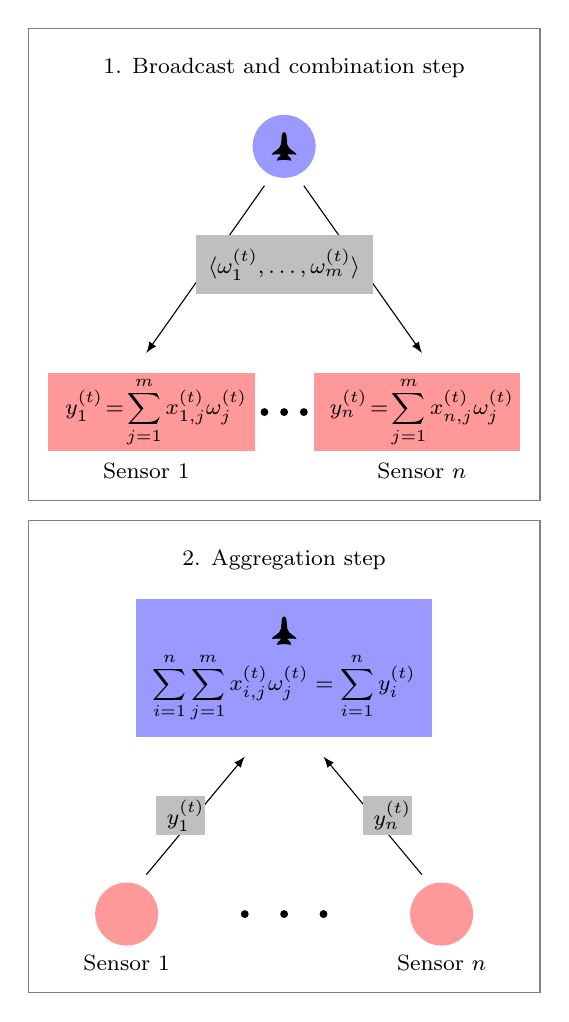
\begin{tikzpicture}[font=\footnotesize]
    % Step 1
    \node at (3.25,5.5) {1. Broadcast and combination step};
    % Navigator
    \fill (3.25,4.5) [blue!40] ellipse (0.4 and 0.4);
    \pic[xscale=0.22,yscale=0.3] at (3.25,4.6725) {plane};
    % Sensors
    \node at (1.5,0.375) {Sensor $1$};
    \fill [red!40] (0.25,0.625) rectangle (2.875,1.625);
    \node at (1.625,1.125) {$\displaystyle y_1^{(t)} \!=\! \sum^m_{j=1}x_{1,j}^{(t)}\omega_j^{(t)}$};
    \node at (5,0.375) {Sensor $n$};
    \fill [red!40] (3.625,0.625) rectangle (6.25,1.625);
    \node at (5,1.125) {$\displaystyle y_n^{(t)} \!=\! \sum^m_{j=1}x_{n,j}^{(t)}\omega_j^{(t)}$};
    \fill [black] (3.5,1.125) circle (0.05);
    \fill [black] (3,1.125) circle (0.05);
    \fill [black] (3.25,1.125) circle (0.05);
    % Lines
    \draw [-latex] plot[smooth, tension=.7] coordinates {(3.5,4) (5,1.875)};
    \draw [-latex] plot[smooth, tension=.7] coordinates {(3,4) (1.5,1.875)};
    \fill [lightgray] (2.125,3.375) rectangle (4.375,2.625);
    \node at (3.25,3) {$\langle\omega_1^{(t)},\dots ,\omega_m^{(t)}\rangle$};
    
    % Step 2
    \node at (3.25,-0.75) {2. Aggregation step};
    % Navigator
    \fill [blue!40] (1.375,-3) rectangle (5.125,-1.25);
    \pic[xscale=0.22,yscale=0.3] at (3.25,-1.4775) {plane};
    \node at (3.25,-2.375) {$\displaystyle \sum^{n}_{i=1}\sum^{m}_{j=1} x_{i,j}^{(t)}\omega_j^{(t)} = \sum^n_{i=1}y^{(t)}_{i}$};
    % Sensors
    \node at (1.25,-5.875) {Sensor $1$};
    \fill  (5.25,-5.25) [red!40] ellipse (0.4 and 0.4);
    \node at (5.25,-5.875) {Sensor $n$};
    \fill  (1.25,-5.25) [red!40] ellipse (0.4 and 0.4);
    \fill [black] (2.75,-5.25) circle (0.05);
    \fill [black] (3.75,-5.25) circle (0.05);
    \fill [black] (3.25,-5.25) circle (0.05);
    % Lines
    \draw [-latex] plot[smooth, tension=.7] coordinates {(5,-4.75) (3.75,-3.25)};
    \draw [-latex] plot[smooth, tension=.7] coordinates {(1.5,-4.75) (2.75,-3.25)};
    \fill [lightgray] (1.625,-3.75) rectangle (2.25,-4.25);
    \node at (2,-4) {$y_1^{(t)}$};
    \fill [lightgray] (4.25,-3.75) rectangle (4.875,-4.25);
    \node at (4.625,-4) {$y_n^{(t)}$};
    
    % Bounding rectangles
    \draw [gray] (0,6) rectangle (6.5,0);
    \draw [gray] (0,-0.25) rectangle (6.5,-6.25);
\end{tikzpicture}
\vspace{\baselineskip}
\caption{Required linear-combination aggregation steps at instance $t$.}
\label{fig:agg_steps}
\end{figure}

In Section \ref{sec:priv_localisation} we will show how this protocol is sufficient to compute the required estimation information at the sensors required to update the navigator's estimation filter.

\begin{rem}
    From the aggregation definition above and the distributive property of real numbers, it is clear that an alternative method to the bi-directional communication requirement would be computing $\sum^{m}_{j=1}\omega_j^{(t)}\sum^{n}_{i=1} x_{i,j}^{(t)}$ by the navigator, requiring only uni-directional communication by sending values $x_{i,j}^{(t)}, 1 \leq j \leq m$ from each sensor $i$. We justify the use of bi-directional communication by reducing communication costs when the number of weights is larger than the number of sensors, $m>n$, and by sending fewer weights in the presence of repeats, as will be shown to be the case in Section \ref{subsec:algorithm}.
\end{rem}

% 
%  ######     ###    ########     ###    ########  #### ##       #### ######## #### ########  ######  
% ##    ##   ## ##   ##     ##   ## ##   ##     ##  ##  ##        ##     ##     ##  ##       ##    ## 
% ##        ##   ##  ##     ##  ##   ##  ##     ##  ##  ##        ##     ##     ##  ##       ##       
% ##       ##     ## ########  ##     ## ########   ##  ##        ##     ##     ##  ######    ######  
% ##       ######### ##        ######### ##     ##  ##  ##        ##     ##     ##  ##             ## 
% ##    ## ##     ## ##        ##     ## ##     ##  ##  ##        ##     ##     ##  ##       ##    ## 
%  ######  ##     ## ##        ##     ## ########  #### ######## ####    ##    #### ########  ######  
% 

\subsection{Participant Capabilities} \label{subsec:capabilities}
Before we can define concrete security requirements and a filtering protocol, we require some assumptions on the capabilities of the navigator and sensors in our problem scenario.
\begin{description}
    \item[Global navigator broadcast] From the decomposition defined above, we know that bi-directional communication between navigator and sensors is required. We make the assumption that broadcast information from the navigator is received by \textit{all} sensors involved in the protocol.
    
    A problem caused by this requirement is apparent in the context of aircraft navigation. It may be the case that some sensors are not within the range of a navigator broadcast. We loosely propose that this scenario can be handled with pre-defined sensor subsets during an initial step by a trusted party. An example has been shown in Figure \ref{fig:sensor_subsets}, which reduces to two separate localisation instances with global broadcasts.
    \item[Consistent navigator broadcast] Further, we make the assumption that broadcast information from the navigator is received equal by all sensors. This means the navigator may not send different information to individual sensors during a single time-step.
    
    In the context of wireless communication, the wide-spread use of cheap non-directional antennas make this assumption reasonable.
    \item[Honest-but-curious sensors] We adopt the honest-but-curious attacker model for all involved sensors, meaning they are assumed to follow the localisation procedure correctly but may store or use any gained sensitive information. 
    
    Misbehaving sensors are a known problem in estimation theory, often requiring inconsistency or outlier detection mechanisms \cite{lazosSeRLocSecureRangeindependent2004,ben-galOutlierDetection2005}. As privacy-preserving implementations of such mechanisms require additional complications, we will not consider the scenario in this work.
    \item[Computational capabilities] The computational requirements for computing encryptions and homomorphic operations are typically more costly than their plaintext equivalents. We make the implicit assumption that all involved parties are computationally capable of computing the required encryption and filter operations.
\end{description}
\begin{figure}[htbp]
\centering
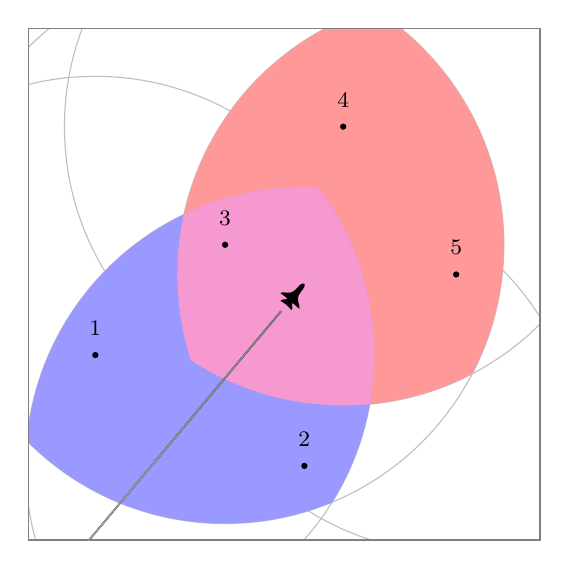
\begin{tikzpicture}[font=\footnotesize]
    % Sizes
    \tikzmath{\srange = 3.54; \sradius = 0.04;}
    % Sensor locations (sensor 3 is shared)
    \coordinate (s1) at (0.8523,-4.1508) {};
    \coordinate (s2) at (3.507,-5.5587) {};
    \coordinate (s3) at (2.5,-2.75) {} {};
    \coordinate (s4) at (4,-1.25) {};
    \coordinate (s5) at (5.4346,-3.1274) {};
    % Navigator location
    \coordinate (nav_loc) at (3.5,-3.25) {};
    % Bounding rectangle
    \coordinate (brect_start) at (0,0);
    \coordinate (brect_end) at (6.5, -6.5);
    
    % Gray range circles
    \begin{scope}
        \clip (brect_start) rectangle (brect_end);
        \draw[gray!50] (s1) circle (\srange);
        \draw[gray!50] (s2) circle (\srange);
        \draw[gray!50] (s3) circle (\srange);
        \draw[gray!50] (s4) circle (\srange);
        \draw[gray!50] (s5) circle (\srange);
    \end{scope}
    % Red subgroup overlap
    \begin{scope}
        \clip (brect_start) rectangle (brect_end);
        \clip (s3) circle (\srange);
        \clip (s4) circle (\srange);
        \clip (s5) circle (\srange);
        \fill[red!40] (brect_start) rectangle (brect_end);
    \end{scope}
    % Blue subgroup overlap
    \begin{scope}
        \clip (brect_start) rectangle (brect_end);
        \clip (s1) circle (\srange);
        \clip (s2) circle (\srange);
        \clip (s3) circle (\srange);
        \fill[blue!40] (brect_start) rectangle (brect_end);
    \end{scope}
    % Magenta double overlap
    \begin{scope}
        \clip (brect_start) rectangle (brect_end);
        \clip (s1) circle (\srange);
        \clip (s2) circle (\srange);
        \clip (s3) circle (\srange);
        \clip (s4) circle (\srange);
        \clip (s5) circle (\srange);
        \fill[magenta!40] (brect_start) rectangle (brect_end);
    \end{scope}
    % Sensors
    \fill[black] (s1) circle (\sradius);
    \fill[black] (s2) circle (\sradius);
    \fill[black] (s3) circle (\sradius);
    \fill[black] (s4) circle (\sradius);
    \fill[black] (s5) circle (\sradius);
    % Bounding box
    \draw[gray] (brect_start) rectangle (brect_end);
    % Navigator
    \clip (brect_start) rectangle (brect_end);
    \pic[rotate=-40,xscale=0.22,yscale=0.3] at (nav_loc) {plane};
    \begin{scope}[shift={(nav_loc)},rotate=-40,xscale=0.22,yscale=0.3]
        % Trail
        \fill[bottom color=white, top color=gray] (-0.05, -1.5) rectangle (0.05, -50);
    \end{scope}
    % Sensor labels
    \node[label=1] at (s1) {};
    \node[label=2] at (s2) {};
    \node[label=3] at (s3) {};
    \node[label=4] at (s4) {};
    \node[label=5] at (s5) {};
\end{tikzpicture}
\caption{An example of sensor subsets. Subsets $\{1,2,3\}$ and $\{3,4,5\}$ can be used independently for localisation when the navigator is within their ranges.}
\label{fig:sensor_subsets}
\end{figure}

% 
% ##       ########    ###    ##    ##    ###     ######   ######## 
% ##       ##         ## ##   ##   ##    ## ##   ##    ##  ##       
% ##       ##        ##   ##  ##  ##    ##   ##  ##        ##       
% ##       ######   ##     ## #####    ##     ## ##   #### ######   
% ##       ##       ######### ##  ##   ######### ##    ##  ##       
% ##       ##       ##     ## ##   ##  ##     ## ##    ##  ##       
% ######## ######## ##     ## ##    ## ##     ##  ######   ######## 
% 

\subsection{Inherent Leakage}
Leakage of information will be discussed in more detail in Section \ref{subsec:leakage}, however, we stress that in any estimation problem where process and measurement models are known, knowledge of sequential state estimates as is the case at the navigator, or the knowledge of one or more measurements as is the case by one or more malicious sensors, naturally leads to the leakage of some information. For this reason, we accept that average sensor information may be leaked to the navigator and that less accurate estimates of location may be leaked to sensors. We will Instead show that individual sensor information remains private to sensors and that the most precise localisation estimate, requiring all measurements, remains private to the navigator. 

% 
% 8888888888 888b    888  .d8888b.       8888888b.  8888888b.  8888888888 888      8888888 888b     d888 
% 888        8888b   888 d88P  Y88b      888   Y88b 888   Y88b 888        888        888   8888b   d8888 
% 888        88888b  888 888    888      888    888 888    888 888        888        888   88888b.d88888 
% 8888888    888Y88b 888 888             888   d88P 888   d88P 8888888    888        888   888Y88888P888 
% 888        888 Y88b888 888             8888888P"  8888888P"  888        888        888   888 Y888P 888 
% 888        888  Y88888 888    888      888        888 T88b   888        888        888   888  Y8P  888 
% 888        888   Y8888 Y88b  d88P      888        888  T88b  888        888        888   888   "   888 
% 8888888888 888    Y888  "Y8888P"       888        888   T88b 8888888888 88888888 8888888 888       888 
%                                                                                                        
%                                                                                                        
%                                                                                                        
% 

\section{Cryptography Preliminaries} \label{sec:crypto_prelim}
When defining our aggregation security requirements and encryption scheme, we will reference some existing cryptographic security notions, the additively homomorphic Paillier encryption scheme and the Joye-Libert private aggregation scheme.

% 
%  ######  ########  ######  ##     ## ########  #### ######## ##    ## 
% ##    ## ##       ##    ## ##     ## ##     ##  ##     ##     ##  ##  
% ##       ##       ##       ##     ## ##     ##  ##     ##      ####   
%  ######  ######   ##       ##     ## ########   ##     ##       ##    
%       ## ##       ##       ##     ## ##   ##    ##     ##       ##    
% ##    ## ##       ##    ## ##     ## ##    ##   ##     ##       ##    
%  ######  ########  ######   #######  ##     ## ####    ##       ##    
% 

\subsection{Security Notions}
The security of a cryptographic scheme is typically defined by a security \textit{game}, which captures both the desired privacy guarantees, as well as the capabilities of attackers \cite{katzIntroductionModernCryptography2008}. The typical security notion for a homomorphic encryption scheme is Indistinguishability under Chosen Plaintext Attack (IND-CPA) \cite{chaseSecurityHomomorphicEncryption2017}. 
\begin{defn}
An encryption scheme meets IND-CPA security if an attacker who can choose plaintext messages to be encrypted at will, gains no additional information about an unknown plaintext message when they learn only its encryption. 

The formal security game for IND-CPA has been given in Appendix \ref{app:ind_cpa}.
\end{defn}
Private aggregation schemes aim for the security notion of Aggregator Obliviousness (AO) \cite{shiPrivacyPreservingAggregationTimeSeries2011}. 
\begin{defn}
An encryption scheme meets AO security if no colluding subset of participants \textit{excluding} the aggregator gains additional information about the remaining aggregation values given only their encryptions, while any colluding subset \textit{including} the aggregator learns only their sum. 

The formal security game for AO has been given in Appendix \ref{app:ao}.
\end{defn}

% 
% ########     ###    #### ##       ##       #### ######## ########  
% ##     ##   ## ##    ##  ##       ##        ##  ##       ##     ## 
% ##     ##  ##   ##   ##  ##       ##        ##  ##       ##     ## 
% ########  ##     ##  ##  ##       ##        ##  ######   ########  
% ##        #########  ##  ##       ##        ##  ##       ##   ##   
% ##        ##     ##  ##  ##       ##        ##  ##       ##    ##  
% ##        ##     ## #### ######## ######## #### ######## ##     ## 
% 

\subsection{Paillier Encryption Scheme} \label{subsec:paillier_scheme}
The Paillier encryption scheme \cite{paillierPublicKeyCryptosystemsBased1999} is an additively homomorphic encryption scheme which bases its security on the decisional composite residuosity assumption (DCRA) and meets the security notion of IND-CPA. Key generation of the Paillier scheme is performed by choosing two sufficiently large primes $p$ and $q$, and computing $N=pq$. A generator $g$ is also required for encryption, which is often set to $g=N+1$ when $p$ and $q$ are of equal bit length \cite{katzIntroductionModernCryptography2008}. The public key is defined by $(N, g)$ and secret key by $(p, q)$.

Encryption of a plaintext message $m \in \mathbb{Z}_N$, producing ciphertext $c \in \mathbb{Z}^{*}_{N^2}$, is computed by
\begin{equation}
    c = g^m r^N \pmod{N^2}
\end{equation}
for a randomly chosen $r \in \mathbb{Z}_{N}$. $r^N$ can be considered the noise term which hides the value $g^m \pmod{N^2}$, which due to the scheme construction, is an easily computable discrete logarithm. The decryption of a ciphertext is computed by
\begin{equation}
    m = \frac{L(c^\lambda\pmod{N^2})}{L(g^\lambda\pmod{N^2})} \pmod{N}
\end{equation}
where $\lambda = \mathsf{lcm}(p-1, q-1)$ and $L(u) = \frac{u-1}{N}$.

In addition to encryption and decryption, the following homomorphic functions are provided by the Paillier scheme. $\forall m_1,m_2 \in \mathbb{Z}_N$,
\begin{align}
    \mathcal{D}(\mathcal{E}(m_1)\mathcal{E}(m_2) \hspace{-7pt} \pmod{N^2}) &= m_1+m_2 \hspace{-7pt} \pmod{N} \\
    \mathcal{D}(\mathcal{E}(m_1)g^{m_2} \hspace{-7pt} \pmod{N^2}) &= m_1+m_2\hspace{-7pt}\pmod{N} \label{eqn:paillier_hom_plain_add}\\
    \mathcal{D}(\mathcal{E}(m_1)^{m_2} \hspace{-7pt} \pmod{N^2}) &= m_1m_2 \hspace{-7pt} \pmod{N}\,. \label{eqn:paillier_hom_mult}
\end{align}

% 
%       ##         ##    ## 
%       ##          ##  ##  
%       ##           ####   
%       ## #######    ##    
% ##    ##            ##    
% ##    ##            ##    
%  ######             ##    
% 

\subsection{Joye-Libert Private Aggregation Scheme} \label{subsec:joye_libert_scheme}
The Joye-Libert private aggregation scheme \cite{joyeScalableSchemePrivacyPreserving2013} is a scheme defined on time-series data, that we refer to as instances for consistency, and meets the security notion of AO. Similarly to the Paillier scheme, it bases its security on the DCRA. A notable difference to a public-key encryption scheme is the need for a trusted party to perform an initial key generation and distribution step.

Key generation is computed by choosing two equal length and sufficiently large primes $p$ and $q$, and computing $N=pq$. Additionally, hash function $H:\mathbb{Z} \rightarrow \mathbb{Z}_{N^2}^*$ is defined, and the public key is set to $(N, H)$. $n$ private keys are generated by choosing $sk_i,\,1\leq i\leq n$ uniformly from $\mathbb{Z}_{N^2}$ and distributing them to all $n$ users (whose values are to be aggregated), while the last key is set as
\begin{equation}
    sk_0 = -\sum^{n}_{i=1}sk_i \pmod{N^2}\,,
\end{equation}
and sent to the aggregator.

Encryption of plaintext $m^{(t)}_{i} \in \mathbb{Z}_N$ to ciphertext $c^{(t)}_{i} \in \mathbb{Z}_{N^2}$ at instance $t$ is computed by user $i$ as
\begin{equation}
    c^{(t)}_{i} = (N+1)^{m^{(t)}_{i}} H(t)^{sk_i} \pmod{N^2}\,,
\end{equation}
where the $H(t)^{sk_i}$ can be considered the noise term which hides the again easily computable discrete logarithm $g^{m^{(t)}_{i}} \pmod{N^2}$, where $g=N+1$.

When all encryptions $c^{(t)}_{i},\,1\leq i \leq n$ are sent to the aggregator, summation and decryption are computed by the functions
\begin{equation}
    c^{(t)} = H(t)^{sk_0}\prod^{n}_{i=1}c^{(t)}_{i} \pmod{N^2}
\end{equation}
and
\begin{equation}
    \sum^{n}_{i=1}m^{(t)}_{i} = \frac{c^{(t)}-1}{N}\,. \label{eqn:agg_decryption}
\end{equation}
Correctness follows from $\sum^{n}_{i=0}sk_i = 0$, and thus
\begin{equation*}
    \begin{split}
        &H(t)^{sk_0}\prod^{n}_{i=1}c_{i,t} \pmod{N^2} \\
        \equiv &H(t)^{sk_0}\prod^{n}_{i=1}(N+1)^{m_{i,t}} H(t)^{sk_i} \pmod{N^2} \\
        \equiv &H(t)^{\sum^n_{j=0}sk_j} \prod^{n}_{i=1}g^{m_{i,t}} \pmod{N^2} \\
        \equiv &(N+1)^{\sum^n_{i=1}m_{i,t}} \pmod{N^2}
    \end{split}
\end{equation*}
removing all noise terms.

% 
% 8888888888 888b    888  .d8888b.       8888888b.  8888888b.   .d88888b.  888888b.   
% 888        8888b   888 d88P  Y88b      888   Y88b 888   Y88b d88P" "Y88b 888  "88b  
% 888        88888b  888 888    888      888    888 888    888 888     888 888  .88P  
% 8888888    888Y88b 888 888             888   d88P 888   d88P 888     888 8888888K.  
% 888        888 Y88b888 888             8888888P"  8888888P"  888     888 888  "Y88b 
% 888        888  Y88888 888    888      888        888 T88b   888     888 888    888 
% 888        888   Y8888 Y88b  d88P      888        888  T88b  Y88b. .d88P 888   d88P 
% 8888888888 888    Y888  "Y8888P"       888        888   T88b  "Y88888P"  8888888P"  
%                                                                                     
%                                                                                     
%                                                                                     
% 

\section{Private Linear-Combination Aggregation} \label{sec:lcao_definition}
As stated in Section \ref{subsec:problem_decomposition}, we decompose the localisation method such that the multi-party aggregation protocol, given in Figure \ref{fig:agg_steps}, captures all communication between the navigator and sensors. To perform this protocol in a secure manner, we must first describe the security properties we aim to achieve during aggregation. Broadly speaking, we want a cryptographic scheme which allows instances of homomorphically computed linear combinations of encrypted weights, to be summed by a private aggregation scheme. That is, we do not want sensors to learn the navigator weights, while we do not want the navigator to learn individual weighted linear combinations. This can be summarised by the two informal security notions:
\begin{description}
    \item[Indistinguishable Weights] No colluding subset of sensors gains any additional knowledge about the navigator weights $\omega_j,\,1\leq j \leq m$ from receiving only their encryptions from the current and previous instances, and the ability to encrypt plaintexts of their choice.
    \item[Private Linear-Combination Aggregation] No colluding subset \textit{excluding} the aggregator gains additional information about the remaining sensor values to be weighted $x^{(t)}_{i,j},\,1\leq j\leq m$, where sensor $i$ is not colluding, given only encryptions of their linear combinations $y_i$ from the current and previous instances. Any colluding subset \textit{including} the aggregator learns only the sum of all linear combinations weighted by weights of their choice, $\sum^{n}_{i=1}y_i^{(t)}=\sum^{n}_{i=1}\sum^{m}_{j=1} x^{(t)}_{i,j}\omega^{(t)}_j$.
\end{description}

\begin{rem} \label{rem:lcao_leakage}
    The notion of a leakage function including parameters from the aggregator requires extra care to be taken when giving its definition. Since an attacker may compromise the aggregator, they have control over the choice of these parameters, and therefore over the leakage function. We note that in the leakage function above, $\sum^n_{i=n}\sum^m_{j=1}x^{(t)}_{i,j}\omega^{(t)}_j$, an individual sum weighted by the same weight may be learned by the colluding subset, \textit{e.g.} $\sum^m_{j=1}x^{(t)}_{i,j}$ given weights $(1,0,\dots,0)$, but that individual sensor values $x^{(t)}_{i,j}$ remain private due to the requirement that all sensors receive the same weights.
\end{rem}

From the informal definitions above, it is clear that weights encrypted by an IND-CPA secure encryption scheme are sufficient for the first requirement, while a scheme satisfying AO is not sufficient for the second. To formalise the second requirement, we define a novel encryption type ``Linear-Combination Aggregator Oblivious Encryption'' and an accompanying security game, which capture the additional weights and modified leakage of AO.

% 
% ##        ######     ###     #######  
% ##       ##    ##   ## ##   ##     ## 
% ##       ##        ##   ##  ##     ## 
% ##       ##       ##     ## ##     ## 
% ##       ##       ######### ##     ## 
% ##       ##    ## ##     ## ##     ## 
% ########  ######  ##     ##  #######  
% 

\subsection{Linear-Combination Aggregator Oblivious Encryption} \label{subsec:lcao}
We let a linear-combination aggregator oblivious encryption scheme be defined as a tuple of the four algorithms $(\mathsf{Setup}, \mathsf{Enc}, \mathsf{CombEnc}, \mathsf{AggDec})$. These are used by a trusted third party, an aggregator and value producing users $i\,1\leq i \leq n$. They are defined as follows

\begin{description}
    \item[$\mathsf{Setup}(\kappa)$] On input of security paramater $\kappa$, generate public parameters $\mathsf{pub}$, the number of weights $m$, the aggregator's public and private keys $pk_0$ and $sk_0$, and the user private keys $sk_i,\,1\leq i \leq n$.
    \item[$\mathsf{Enc}(pk_0, a)$] The aggregator and users can encrypt any value $a$ with the aggregator public key $pk_0$, and obtain the encryption $\mathcal{E}_{pk_0}(a)$.
    \item[$\mathsf{CombEnc}(t, pk_0, sk_i, \mathcal{E}_{pk_0}(\omega_1^{(t)}),\dots,\mathcal{E}_{pk_0}(\omega_m^{(t)}), x^{(t)}_{i,1},\dots,x^{(t)}_{i,m})$] At instance $t$, user $i$ computes and obtains the encrypted linear combination $y^{(t)}_i = \mathcal{E}_{pk_0,sk_i}(\sum^m_{j=1}x^{(t)}_{i,j}\omega^{(t)}_j)$ using its secret key $sk_i$.
    \item[$\mathsf{AggDec}(t, pk_0, sk_0, y^{(t)}_1,\dots,y^{(t)}_n)$] At instance $t$, the aggregator computes the aggregation of linear combinations $\sum^{n}_{i=1}y_i^{(t)}=\sum^{n}_{i=1}\sum^{m}_{j=1} x^{(t)}_{i,j}\omega^{(t)}_j$ using its public and private keys $pk_0$, $sk_0$.
\end{description}

We formalise the security notion of Linear-Combination Aggregator Obliviousness (LCAO) as the following game between attacker and challenger:

\begin{description}
    \item[Setup] The challenger runs the $\mathsf{Setup}$ algorithm and gives $\mathsf{pub}$, $m$ and $pk_0$ to the attacker
    \item[Queries] The attacker can now perform encryptions or submit queries that are answered by the challenger. The types of actions are:
    \begin{enumerate}
        \item \textit{Encryption:} The attacker chooses a value $a$ and computes an encryption of $a$ under the aggregator's public key $pk_0$, obtaining $\mathcal{E}_{pk_0}(a)$.
        \item \textit{Weight Queries:} The attacker chooses an instance $t$ and receives the weights for that instance encrypted with the aggregator's public key, $\mathcal{E}_{pk_0}(\omega^{(t)}_{j}),\,1\leq j\leq m$.
        \item \textit{Combine Queries:} The attacker chooses a tuple $(i,t,x^{(t)}_{i,1},\dots,x^{(t)}_{i,m})$ such that for any two chosen combine query tuples $(i,t,x^{(t)}_{i,1},\dots,x^{(t)}_{i,m})$ and $(i',t',x^{\prime(t')}_{i',1},\dots,x^{\prime(t')}_{i',m})$, the following condition holds:
        \begin{equation*}
            i = i' \wedge t = t' \implies x^{(t)}_{i,m} = x^{\prime(t')}_{i',m},\,1\leq j\leq m\,.
        \end{equation*}
        The attacker is then given back the encryption of the linear combination $\mathcal{E}_{pk_0,sk_i}(\sum^m_{j=1}x^{(t)}_{i,j}\omega^{(t)}_j)$ encrypted under both the aggregator public key $pk_0$ and the secret key $sk_i$.
        \item \textit{Compromise queries:} The attacker chooses $i$ and receives the secret key $sk_i$. The aggregator's secret key may also be compromised (when choosing $i=0$).
    \end{enumerate} 
    \item[Challenge] Next, the attacker chooses an instance $t^*$, and a subset of users $S \subseteq U$ where $U$ is the complete set of users for which no combine queries, for the instance $t^*$, and no compromise queries, are made for the duration of the game. The attacker then chooses two series of tuples
    \begin{equation*}
        \langle(i,t^*,x^{(t^*)(0)}_{i,1},\dots,x^{(t^*)(0)}_{i,m})\,|\,i \in S\rangle
    \end{equation*}
    and
    \begin{equation*}
        \langle(i,t^*,x^{(t^*)(1)}_{i,1},\dots,x^{(t^*)(1)}_{i,m})\,|\, i \in S\rangle\,,
    \end{equation*}
    and gives them to the challenger. In the case that $0 \in S$ (\textit{i.e.} the aggregator is compromised) and $S = U$, it is additionally required that
    \begin{equation*}
        \sum_{i\in S}\sum^{m}_{j=1} x^{(t^*)(0)}_{i,j}\omega^{(t^*)}_j = \sum_{i \in S}\sum^{m}_{j=1} x^{(t^*)(1)}_{i,j}\omega^{(t^*)}_j\,,
    \end{equation*}
    for weights $\omega^{(t^*)}_j,\,1\leq j \leq m$ returned by a \textit{Weight Query} with chosen instance $t^*$. The challenger then chooses a random bit $b \in \{1,0\}$ and returns encryptions 
    \begin{equation*}
        \langle\mathcal{E}_{pk_0,sk_i}(\sum^m_{j=1}x^{(t^*)(b)}_{i,j}\omega^{(t^*)}_j)\,|\,i\in S\rangle\,.
    \end{equation*}
    \item[More Queries] The attacker can now perform more encryptions and submit queries, so long as the queries do not break the requirements in the Challenge stage. That is, $S \subseteq U$.
    \item[Guess] At the end, the attacker outputs a bit $b'$ and wins the game if and only if $b' = b$. The advantage of an attacker $\mathcal{A}$ is defined as
    \begin{equation*}
        \mathsf{Adv}^{LCAO}(\mathcal{A}) \coloneqq \left\lvert \Pr [b'=b] - \frac{1}{2}\right\rvert\,.
    \end{equation*} 
\end{description}

\begin{defn}
    An encryption scheme meets LCAO security if no adversary, running in probabilistic-time with respect to security parameter, has more than a negligible advantage in winning the above security game. Probabilities are taken over randomness introduced by $\mathcal{A}$, and in $\mathsf{Setup}$, $\mathsf{Enc}$ and $\mathsf{CombEnc}$.
\end{defn}

In the next section, we will give a solution to an encryption scheme meeting LCAO security, with IND-CPA secure weight encryption, and give a cryptographic proof for its security.

% 
%  #######  ##     ## ########      ######   ######  ##     ## ######## ##     ## ######## 
% ##     ## ##     ## ##     ##    ##    ## ##    ## ##     ## ##       ###   ### ##       
% ##     ## ##     ## ##     ##    ##       ##       ##     ## ##       #### #### ##       
% ##     ## ##     ## ########      ######  ##       ######### ######   ## ### ## ######   
% ##     ## ##     ## ##   ##            ## ##       ##     ## ##       ##     ## ##       
% ##     ## ##     ## ##    ##     ##    ## ##    ## ##     ## ##       ##     ## ##       
%  #######   #######  ##     ##     ######   ######  ##     ## ######## ##     ## ######## 
% 

\subsection{Our Scheme} \label{subsec:our_scheme}
Our scheme is based on the Paillier and Joye-Libert schemes introduced in Sections \ref{subsec:paillier_scheme} and \ref{subsec:joye_libert_scheme}, and similarly bases its security on the DCRA. As with Joye-Libert's private aggregation scheme, a trusted party is required for the initial distribution of user secret keys. Below, we give definitions for the four algorithms comprising the linear-combination aggregation encryption scheme.

\begin{description}
    \item[$\mathsf{Setup}(\kappa)$] On input parameter $\kappa$, generate two equal length, sufficiently large, primes $p$ and $q$, and compute $N=pq$. Define a hash function $H:\mathbb{Z} \rightarrow \mathbb{Z}_{N^2}^*$, choose an $m>1$ as the number of weights to combine, and set public parameter $\mathsf{pub}=H$, aggregator public key $pk_0 = N$ and aggregator private key $sk_0=(p,q)$. The remaining user secret keys are generated by choosing $sk_i,\,1\leq i\leq n-1$ uniformly from $\mathbb{Z}_{N^2}$ and setting the last key as $sk_n = -\sum^{n-1}_{i=1}sk_i \pmod{N^2}$.
 
    \item[$\mathsf{Enc}(pk_0, a)$] Encryption of values is computed as a Paillier encryption with implicit generator $g=N+1$. This is given by
    \begin{equation}
        \mathcal{E}_{pk_0}(a) = (N+1)^{a}r^N \pmod{N^2}\,, \label{eqn:our_scheme_encrypt}
    \end{equation}
    for a randomly chosen $r \in \mathbb{Z}_N$.

    \item[$\mathsf{CombEnc}(t, pk_0, sk_i, \mathcal{E}_{pk_0}(\omega_1^{(t)}),\dots,\mathcal{E}_{pk_0}(\omega_m^{(t)}), x^{(t)}_{i,1},\dots,x^{(t)}_{i,m})$] The linear combination encryption step at instance $t$ is computed as 
    \begin{equation}
        y^{(t)}_i = H(t)^{sk_i}\prod^{m}_{j=1}\mathcal{E}_{pk_0}(\omega^{(t)}_j)^{x^{(t)}_{i,j}} \pmod{N^2}\,,\label{eqn:our_scheme_lin_comb}
    \end{equation}
    and makes use of the homomorphic property \eqref{eqn:paillier_hom_mult}. Correctness follows from
    \begin{equation*}
        \begin{split}
             y^{(t)}_i &= H(t)^{sk_i}\prod^{m}_{j=1}\mathcal{E}_{pk_0}(\omega^{(t)}_j)^{x^{(t)}_{i,j}} \pmod{N^2} \\
            &= H(t)^{sk_i}\prod^{m}_{j=1}\mathcal{E}_{pk_0}(x^{(t)}_{i,j}\omega^{(t)}_j) \pmod{N^2} \\
            &= H(t)^{sk_i}\prod^{m}_{j=1}(N+1)^{x^{(t)}_{i,j}\omega^{(t)}_j} r^{N}_{j} \pmod{N^2} \\
            &= H(t)^{sk_i}(N+1)^{\sum^{m}_{j=1}x^{(t)}_{i,j}\omega^{(t)}_j} r_{i}^{N} \pmod{N^2}\,,
        \end{split}
    \end{equation*}
    for some values $r_i,r_j \in \mathbb{Z}_N\,,1\leq j \leq m$. Here, $r_i^N$ and $H(t)^{sk_i}$ can be considered the noise terms corresponding to the two levels of encryption from $pk_0$ and $sk_i$, respectively.

    \item[$\mathsf{AggDec}(t, pk_0, sk_0, y^{(t)}_1,\dots,y^{(t)}_n)$] Aggregation is computed as $y^{(t)} = \prod^n_{i=1}y^{(t)}_i \pmod{N^2}$, removing aggregation noise terms, and is followed by Paillier decryption
    \begin{equation}
        \begin{split}
            \sum^{n}_{i=1}\sum^{m}_{j=1}&x^{(t)}_{i,j}\omega^{(t)}_j =\\
            &\frac{L((y^{(t)})^\lambda\pmod{N^2})}{L((N+1)^\lambda\pmod{N^2})} \pmod{N}\,.
        \end{split} \label{eqn:our_scheme_decrypt}
    \end{equation}
    The correctness of aggregation can be seen from
    \begin{align*}
        y^{(t)} &= \prod^n_{i=1}H(t)^{sk_i}(N+1)^{\sum^{m}_{j=1}x_{i,j}\omega_j}r_i^N \pmod{N^2} \\
        \begin{split}
            &= H(t)^{\sum^n_{i=1}sk_i}\cdot \\
            &\qquad\qquad \prod^n_{i=1}(N+1)^{\sum^{m}_{j=1}x^{(t)}_{i,j}\omega^{(t)}_j}r_i^N \pmod{N^2}
        \end{split}\\
        &= (N+1)^{\sum^n_{i=1}\sum^{m}_{j=1}x^{(t)}_{i,j}\omega^{(t)}_j}r'^N \pmod{N^2}\,,
    \end{align*}
    for some values $r_i,r' \in \mathbb{Z}_N,\,1\leq i \leq n$.
\end{description}

Additionally, we note that in the above construction, all weights $\omega^{(t)}_j$ and values $x^{(t)}_{i,j}$ are integers, and that resulting linear combinations and summations are computed $\pmod{N}$.

\begin{rem} \label{rem:lcao_implicit_weight}
    The construction of this scheme additionally supports the linear combination of the implicit weight, $\omega^{(t)}_j = 1$, by replacing
    \begin{equation}
        \mathcal{E}_{pk_0}(1)^{x^{(t)}_{i,j}} = (N+1)^{1}r_j^N \pmod{N^2}
    \end{equation}
    in \eqref{eqn:our_scheme_lin_comb} by
    \begin{equation}
        (N+1)^{x^{(t)}_{i,j}} \pmod{N^2}\,,
    \end{equation}
    due to the removal of $r_j^N$ terms during decryption. This can be used to reduce the broadcast communication cost by one weight.
\end{rem}

% 
% ########  ########   #######   #######  ######## 
% ##     ## ##     ## ##     ## ##     ## ##       
% ##     ## ##     ## ##     ## ##     ## ##       
% ########  ########  ##     ## ##     ## ######   
% ##        ##   ##   ##     ## ##     ## ##       
% ##        ##    ##  ##     ## ##     ## ##       
% ##        ##     ##  #######   #######  ##       
% 

\subsection{Security Proof}
To prove the security of our introduced scheme, we recall the desired security properties of an LCAO secure scheme with IND-CPA secure encrypted weights. From the definition above, weights encrypted with public key $pk_0$ are identical to encryptions of the Paillier scheme, and therefore meet security notion IND-CPA. We omit this proof here and refer readers to the security proof of the Paillier encryption scheme \cite{paillierPublicKeyCryptosystemsBased1999} instead.

To show our scheme meets the security notion of LCAO, we prove by contrapositive that for an adversary $\mathcal{A}$ playing against a challenger using \textit{our scheme}, we can create an adversary $\mathcal{A}'$ playing against a challenger $\mathcal{C}$ using the \textit{Joye-Libert scheme}, such that
\begin{equation*}
    \mathsf{Adv}^{LCAO}(\mathcal{A}) > \eta_1(\kappa) \implies \mathsf{Adv}^{AO}(\mathcal{A}') > \eta_2(\kappa)\,,
\end{equation*}
for some negligible functions $\eta_1$ and $\eta_2$. (\textit{i.e.} if we assume our scheme is not LCAO secure, then the Joye-Libert scheme is not AO secure.) Given the Joye-Libert AO proof in \cite{joyeScalableSchemePrivacyPreserving2013}, we know our scheme must be LCAO secure and will thus conclude our proof. The proof overview has been given in Figure \ref{fig:proof_summary}. Additionally, the function $H$ used by our scheme is treated as a \textit{random oracle} in the Joye-Libert AO proof and will, therefore, prove our scheme secure in the random oracle model as well.

\begin{figure}[htbp]
\centering
\vspace{\baselineskip}
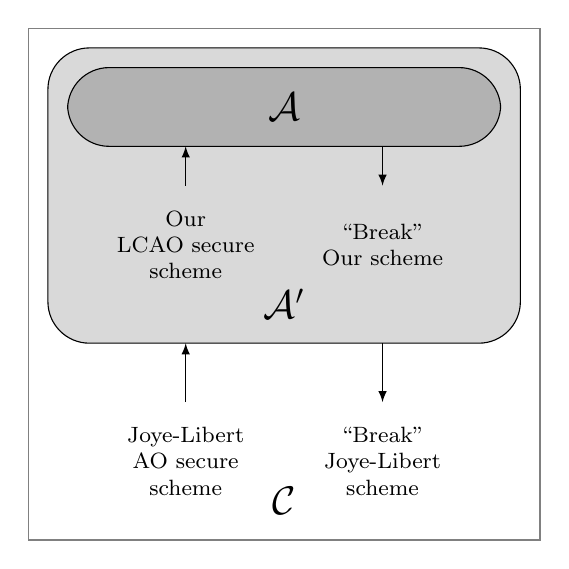
\begin{tikzpicture}[font=\footnotesize]
    % Bounding box
    \draw [gray] (0,0) rectangle (6.5,6.5);

    % Outer adversary rectangle
    \draw[rounded corners=15pt, fill=gray!30] (0.25,6.25) rectangle (6.25,2.5);
    % Inner adversary rectangle
    \draw[rounded corners=15pt, fill=gray!60] (0.5,6) rectangle (6,5);

    % Adversaries and challenger
    \node at (3.25,3) {\Large$\mathcal{A}'$};
    \node at (3.25,5.5) {\Large$\mathcal{A}$};
    \node at (3.25,0.5) {\Large$\mathcal{C}$};

    % Arrows
    \node[text width=3cm, align=center] at (2,1) {Joye-Libert\\AO secure\\scheme};
    \draw [-latex] (2,1.75) -- (2,2.5);

    \node[text width=3cm, align=center] at (2,3.75) {Our\\LCAO secure\\scheme};
    \draw [-latex] (2,4.5) --(2,5);

    \node[text width=3cm, align=center] at (4.5,3.75) {``Break''\\Our scheme};
    \draw [-latex] (4.5,5) -- (4.5,4.5);

    \node[text width=3cm, align=center] at (4.5,1) {``Break''\\Joye-Libert\\scheme};
    \draw [-latex] (4.5,2.5) -- (4.5,1.75);
\end{tikzpicture}
\vspace{\baselineskip}
\caption{High-level overview of our scheme's LCAO security proof.}
\label{fig:proof_summary}
\end{figure}

\begin{pf}
    Consider adversary $\mathcal{A}$ playing the LCAO game defined in Section \ref{subsec:lcao}. The following is a construction of an adversary $\mathcal{A}'$ playing the AO game in Appendix \ref{app:ao} against a challenger $\mathcal{C}$ using the Joye-Libert aggregation scheme from Section \ref{subsec:joye_libert_scheme}.
    \begin{description}
        \item[Setup] When receiving $N$ and $H$ as public parameters from $\mathcal{C}$, choose an $m>1$ and give public parameter $H$, number of weights $m$, and $pk_0=N$ to $\mathcal{A}$.
        \item[Queries] Handle queries from $\mathcal{A}$:
        \begin{description}
            \item[\textit{Weight Query}] When $\mathcal{A}$ submits a weight query $t$, choose weights $\omega^{(t)}_j,\,1 \leq j \leq m$ and random values $r_j \in \mathbb{Z}_N,\,1 \leq j \leq m$, and return encryptions 
            \begin{equation*}
                (N+1)^{\omega^{(t)}_{j}}r_j^N\pmod{N^2},\,1\leq j\leq m
            \end{equation*}
            to $\mathcal{A}$.
            \item[\textit{Combine Query}] When $\mathcal{A}$ submits combine query $(i, t, x^{(t)}_{i,1},\dots,x^{(t)}_{i,m})$, choose weights $\omega^{(t)}_j,1 \leq j \leq m$ if not already chosen for the instance $t$, and make an AO encryption query $(i, t, \sum^m_{j=1}x^{(t)}_{i,j}\omega^{(t)}_j)$ to $\mathcal{C}$. The received response will be of the form $(N+1)^{\sum^m_{j=1}x^{(t)}_{i,j}\omega^{(t)}_j}H(t)^{sk_i}$; multiply it by $r^N$ for a random $r \in \mathbb{Z}_N$ and return 
            \begin{equation*}
                (N+1)^{\sum^m_{j=1}x^{(t)}_{i,j}\omega^{(t)}_j}r^N H(t)^{sk_i} \pmod{N^2}
            \end{equation*}
            to $\mathcal{A}$.
            \item[\textit{Compromise Query}] When $\mathcal{A}$ submits compromise query $i$, make the same compromise query $i$ to $\mathcal{C}$, and return the recieved secret key $sk_i$ to $\mathcal{A}$.
        \end{description}
        \item[Challenge] When $\mathcal{A}$ submits challenge series
        \begin{equation*}
            \langle(i,t^*,x^{(t^*)(0)}_{i,1},\dots,x^{(t^*)(0)}_{i,m})\,|\,i \in S\rangle
        \end{equation*}
        and
        \begin{equation*}
            \langle(i,t^*,x^{(t^*)(1)}_{i,1},\dots,x^{(t^*)(1)}_{i,m})\,|\, i \in S\rangle\,,
        \end{equation*}
        choose weights $\omega^{(t^*)}_j,1 \leq j \leq m$ for instance $t^*$ and submit AO challenge series
        \begin{equation*}
            \langle(i,t^*,\sum^m_{j=1}x^{(t^*)(0)}_{i,j}\omega^{(t^*)}_j)\,|\,i \in S\rangle
        \end{equation*}
        and
        \begin{equation*}
            \langle(i,t^*,\sum^m_{j=1}x^{(t^*)(1)}_{i,j}\omega^{(t^*)}_j)\,|\,i \in S\rangle\,,
        \end{equation*}
        to $\mathcal{C}$. The received response will be of the form 
        \begin{equation*}
            \langle(N+1)^{\sum^m_{j=1}x^{(t^*)(b)}_{i,j}\omega^{(t^*)}_j}H(t^*)^{sk_i}\,|\,i\in U\rangle\,,
        \end{equation*}
        for an unknown $b \in \{0,1\}$. Multiply series elements by $r_i^N,\,1 \leq i \leq n$ for randomly chosen $r_i \in \mathbb{Z}_N$ and return
        \begin{equation*}
            \langle(N+1)^{\sum^m_{j=1}x^{(t^*)(b)}_{i,j}\omega^{(t^*)}_j}r_i^N H(t^*)^{sk_i}\,|\,i\in U\rangle
        \end{equation*}
        to $\mathcal{A}$.
        \item[Guess] When $\mathcal{A}$ makes guess $b'$, make the same guess $b'$ to $\mathcal{C}$.
    \end{description}

    In the above construction, $\mathcal{C}$ follows the Joye-Libert scheme from Section \ref{subsec:joye_libert_scheme} exactly, and to $\mathcal{A}$, $\mathcal{A}'$ follows our scheme in Section \ref{subsec:our_scheme} exactly. Since $\mathcal{A}'$ runs in polynomial-time to security parameter when $\mathcal{A}$ does, and no non-neglibile advantage adversary to $\mathcal{C}$ exists \cite{joyeScalableSchemePrivacyPreserving2013}, we conclude that no non-negligible advantage adversary $\mathcal{A}$ exists. That is, there exists a negligible function $\eta$, such that
    \begin{equation*}
        \mathsf{Adv}^{LCAO}(\mathcal{A}) \leq \eta(\kappa)
    \end{equation*}
    for security parameter $\kappa$. \qed
\end{pf}

% 
% 888      .d88888b.   .d8888b.       8888888b.  8888888b.  8888888888 888      8888888 888b     d888 
% 888     d88P" "Y88b d88P  Y88b      888   Y88b 888   Y88b 888        888        888   8888b   d8888 
% 888     888     888 888    888      888    888 888    888 888        888        888   88888b.d88888 
% 888     888     888 888             888   d88P 888   d88P 8888888    888        888   888Y88888P888 
% 888     888     888 888             8888888P"  8888888P"  888        888        888   888 Y888P 888 
% 888     888     888 888    888      888        888 T88b   888        888        888   888  Y8P  888 
% 888     Y88b. .d88P Y88b  d88P      888        888  T88b  888        888        888   888   "   888 
% 88888888 "Y88888P"   "Y8888P"       888        888   T88b 8888888888 88888888 8888888 888       888 
%                                                                                                     
%                                                                                                     
%                                                                                                     
% 

\section{Encrypted Localisation Preliminaries} \label{sec:loc_prelim}
Our next goal is to apply the LCAO secure encryption scheme introduced to a Bayesian localisation filter. The filter we introduce requires the use of real-valued inputs and functions, and relies on a non-linear measurement model. We will make use of a real-number encoding scheme supporting our required homomorphic operations as well as a reformulated Extended Kalman Filter which reduces the filter update step to use only these operations.

% 
% ######## ##    ##  ######   #######  ########  #### ##    ##  ######   
% ##       ###   ## ##    ## ##     ## ##     ##  ##  ###   ## ##    ##  
% ##       ####  ## ##       ##     ## ##     ##  ##  ####  ## ##        
% ######   ## ## ## ##       ##     ## ##     ##  ##  ## ## ## ##   #### 
% ##       ##  #### ##       ##     ## ##     ##  ##  ##  #### ##    ##  
% ##       ##   ### ##    ## ##     ## ##     ##  ##  ##   ### ##    ##  
% ######## ##    ##  ######   #######  ########  #### ##    ##  ######   
% 

\subsection{Integer Encoding for Real Numbers} \label{subsec:encoding}
In the encryption scheme introduced, weights and values are restricted to integers and all operations are computed $\pmod{N}$, thus bounding meaningful inputs to $\{x \,|\, x \in \mathbb{Z}_N\}$. For this reason, a quantisation and integer mapping method for real numbers is required for their encryption and homomorphic processing. We quantise with a generalised Q number format \cite{oberstarFixedPointRepresentationFractional2007} due to implementation simplicity and applicability.

We define a subset of rational numbers in terms of a range $r \in \mathbb{N}$ and fractional precision $f \in \mathbb{N}$. This contrasts with the common definition given in terms of total bits and fractional bits \cite{oberstarFixedPointRepresentationFractional2007,schulzedarupEncryptedCooperativeControl2019,farokhiSecurePrivateControl2017}, but allows for a direct mapping to integer ranges which are not powers of two. Rational subset $\mathbb{Q}_{r,f}$ is given by
\begin{equation}
    \mathbb{Q}_{r,f} = \left\{q \,|\, f^{-1}\ \textsf{divides}\ q \wedge -\left\lfloor\frac{r}{2}\right\rfloor \leq q < \left\lfloor\frac{r}{2}\right\rfloor \right\}\,,
\end{equation}
and we quantise any real number $x$ by taking the nearest rational $q \in \mathbb{Q}_{r,f}$. That is, $\argmin_{q\in\mathbb{Q}_{r,f}} |x-q|$. In this form, mapping rationals $\mathbb{Q}_{r,f}$ to the encryption scheme range $\mathbb{Z}_N$ is achieved by choosing $r=N$, and handling negatives with modulo arithmetic. In addition, we note that the Q number format requires a precision factor $f$ to be removed after each encoded multiplication, which is not supported by our encryption scheme. This is captured by a third parameter $m$; the number of multiplication factors to add or remove from encodings.

The function for combined quantisation and encoding $\mathsf{E}_{r,f,m}(x)$, of a given a real number $x \in \mathbb{R}$, integer range $\mathbb{Z}_r$, and the desired scaling for $m$ prior encoded multiplications, is given by
\begin{equation}
    \mathsf{E}_{r,f,m}(x) = \left\lfloor f^{m+1} x \right\rceil \pmod{r}\,. \label{eqn:encode}
\end{equation}
Decoding of an integer $e \in \mathbb{Z}_r$, is given by
\begin{equation}
    \mathsf{E}^{-1}_{r,f,m}(e) \!=\! 
    \begin{dcases}
        \frac{e\hspace{-8pt}\pmod{r}}{f^{m+1}}, &e\hspace{-8pt}\pmod{r} \leq \left\lfloor\frac{r}{2}\right\rfloor \\
        -\frac{r - e\hspace{-8pt}\pmod{r}}{f^{m+1}}, &\text{otherwise} \\
    \end{dcases}.\label{eqn:decode}
\end{equation}

This encoding scheme provides the following homomorphic operations,
\begin{equation}
    \begin{split}
        \mathsf{E}_{r,f,m}(a_1) + \mathsf{E}_{r,f,m}(a_2)& \pmod{r} =\\
        &\mathsf{E}_{r,f,m}(a_1+a_2)
    \end{split}\label{eqn:encoding_homomorphic_add}
\end{equation}
and
\begin{equation}
    \begin{split}
        \mathsf{E}_{r,f,m}(a_1)\mathsf{E}_{r,f,m}(a_2)& \pmod{r} =\\
        &\mathsf{E}_{r,f,m+1}(a_1a_2)\,,
    \end{split}
\end{equation}
noting that when $r=N$, the modulus corresponds with the encrypted homomorphic operations in \eqref{eqn:paillier_hom_plain_add}, \eqref{eqn:paillier_hom_mult} and therefore \eqref{eqn:our_scheme_lin_comb}.

The choice of a high fractional precision $f$ may reduce quantisation errors introduced in \eqref{eqn:encode}, however, risks an overflow following too many multiplications. Given the largest number of expected multiplications $m_{max}$, and the largest expected decoded value $x$, the parameter should be chosen such that the following condition holds
\begin{equation}
    \left|f^{m_{max}+1}x\right| < \left\lfloor \frac{r}{2} \right\rfloor\,.
\end{equation}
In practice, $N$ is typically very large ($N>2^{1024}$) and this condition can be ignored when $r=N$.

% 
% ######## #### ######## 
% ##        ##  ##       
% ##        ##  ##       
% ######    ##  ######   
% ##        ##  ##       
% ##        ##  ##       
% ######## #### ##       
% 

\subsection{Extended Information Filter}
The Extended Information Filter (EIF) \cite{maybeckStochasticModelsEstimation1982} is a reformulation of the Extended Kalman Filter (EKF), such that the update equations are simplified to sums of measurement information from each sensor. This requires the conversion of predicted state estimate $\rvec{x}_{k|k-1}$ and estimate covariance $\mat{P}_{k|k-1}$ to the information vector and matrix
\begin{equation}
    \rvec{y}_{k|k-1} = \mat{P}_{k|k-1}^{-1}\rvec{x}_{k|k-1} \quad\textrm{and}\quad \mat{Y}_{k|k-1} = \mat{P}_{k|k-1}^{-1}\,,
\end{equation}
respectively. In this form, the update equations for $n$ measurements at time $k$, given process and measurement models \eqref{eqn:process_model} and \eqref{eqn:measurement_model}, are given by
\begin{equation}
    \begin{split}
        &\rvec{y}_{k|k} = \rvec{y}_{k|k-1} + \\
        &\quad \sum^n_{i=1}\mat{H}^\top_{k,i} r^{-1}_i (z_{k,i} - h_i(\rvec{x}_{k|k-1}) + \mat{H}_{k,i}\rvec{x}_{k|k-1})
    \end{split} \label{eqn:eif_info_vec_update}
\end{equation}
and
\begin{equation}
    \mat{Y}_{k|k} = \mat{Y}_{k|k-1} + \sum^n_{i=1}\mat{H}^\top_{k,i} r^{-1}_i \mat{H}_{k,i}\,, \label{eqn:eif_info_mat_update}
\end{equation}
with Jacobians
\begin{equation}
    \mat{H}_{k,i} = \left.\frac{\partial h_i}{\partial \vec{x}}\right|_{\rvec{x}_{k|k-1}} \label{eqn:measurement_jacobian}
\end{equation}
for sensors $1 \leq i \leq n$. The filter's prediction step can be computed by converting information vector $\rvec{y}_{k|k}$ and matrix $\mat{Y}_{k|k}$ back to state estimate and covariance 
\begin{equation}
    \rvec{x}_{k|k} = \mat{Y}_{k|k}^{-1}\rvec{y}_{k|k} \quad\textrm{and}\quad \mat{P}_{k|k} = \mat{Y}_{k|k}^{-1}\,,
\end{equation}
before using the normal EKF prediction equations
\begin{equation}
    \rvec{x}_{k+1|k} = \vec{f}(\rvec{x}_{k|k})
\end{equation}
and
\begin{equation}
    \mat{P}_{k+1|k} = \mat{F}_k\mat{P}_{k|k}\mat{F}_k^\top\,,
\end{equation}
with Jacobian
\begin{equation}
    \mat{F}_{k} = \left.\frac{\partial \vec{f}}{\partial \vec{x}}\right|_{\rvec{x}_{k|k}}\,. \label{eqn:jacobian_f}
\end{equation}

% 
% 888      .d88888b.   .d8888b.  
% 888     d88P" "Y88b d88P  Y88b 
% 888     888     888 888    888 
% 888     888     888 888        
% 888     888     888 888        
% 888     888     888 888    888 
% 888     Y88b. .d88P Y88b  d88P 
% 88888888 "Y88888P"   "Y8888P"  
%                                
%                                
%                                
% 

\section{Privacy-Preserving Localisation} \label{sec:priv_localisation}
With the relevant preliminaries, we now apply the LCAO secure scheme to our original localisation problem. Recall we are considering a navigator in the presence of $n$ range sensors. The navigator runs a local filter, computing its update step with equations \eqref{eqn:eif_info_vec_update} and \eqref{eqn:eif_info_mat_update}, where received information from each sensor $i$ consists of the measurement vector
\begin{equation}
    \rvec{i}_{k,i} = \mat{H}^\top_{k,i} r^{-1}_i (\rv{z}_{k,i} - h_i(\rvec{x}_{k|k-1}) + \mat{H}_{k,i}\rvec{x}_{k|k-1}) \label{eqn:measurement_vec}
\end{equation}
and the measurement matrix
\begin{equation}
    \mat{I}_{k,i} = \mat{H}^\top_{k,i} r^{-1}_i \mat{H}_{k,i}\,, \label{eqn:measurement_mat}
\end{equation}
at each time-step $k$. In this form, all sensitive sensor information is exclusively found in $\rvec{i}_{k,i}$ and $\mat{I}_{k,i}$. Namely, their measurements $\rv{z}_{k,i}$, measurement variances $r_i$ and locations $\vec{s}_i$; captured in measurement functions $h_i$ and Jacobians $\mat{H}_{k,i}$. 

The reason for using a linear-combination aggregation scheme in this scenario is due to computing $\rvec{i}_{k,i}$ and $\mat{I}_{k,i}$ at the sensors requiring the navigator to disclose some location information in $\rvec{x}_{k|k-1}$, for the computing of Jacobians $\mat{H}_{k,i}$. Instead, we want to reformulate $\rvec{i}_{k,i}$ and $\mat{I}_{k,i}$ such that the sensors can use the LCAO secure scheme, with location information in $\rvec{x}_{k|k-1}$ as weights from the navigator. As was shown in Section \ref{subsec:our_scheme}, this guarantees that sensors cannot learn navigator location information $\rvec{x}_{k|k-1}$, and that the navigator cannot learn individual sensor values required for computing $\rvec{i}_{k,i}$ and $\mat{I}_{k,i}$. From \eqref{eqn:measurement_vec} and \eqref{eqn:measurement_mat} we see that such a linear reformulation will set requirements on the possible measurement functions $h_i$. 

% 
% ##     ##   ### ##     ## ###      ########  ########  #######   ######  
% ##     ##  ##    ##   ##    ##     ##     ## ##       ##     ## ##    ## 
% ##     ## ##      ## ##      ##    ##     ## ##       ##     ## ##       
% ######### ##       ###       ##    ########  ######   ##     ##  ######  
% ##     ## ##      ## ##      ##    ##   ##   ##       ##  ## ##       ## 
% ##     ##  ##    ##   ##    ##     ##    ##  ##       ##    ##  ##    ## 
% ##     ##   ### ##     ## ###      ##     ## ########  ##### ##  ######  
% 

\subsection{Measurement Model Requirements}
From the definition of matrix multiplication, we know that matrices whose elements are linear combinations of weights can be multiplied to produce elements of new linear combinations, with new weights as functions dependant only on weights from the original matrices. For example, consider dimension $N\times N$ matrices $\mat{A}$ and $\mat{B}$, where element $(i,j)$ in matrix $\mat{A}$ is of the form $\sum_{l=0}^M w_{l,i,j}a_{l,i,j}$ and similarly for matrix $\mat{B}$, the form $\sum_{l=0}^M v_{l,i,j}b_{l,i,j}$. If we consider $w_{l,i,j}$ and $v_{l,i,j}$ as the weight terms, we can write element $(i,j)$ of a product matrix $\mat{A}\mat{B}$, as a linear combination of functions dependant only on these weights, as
\begin{equation}
    \begin{split}
        \sum_{l=0}^N&\left(\left(\sum_{m=0}^M w_{m,i,j}a_{m,i,l}\right)\left(\sum_{m=0}^Mv_{m,i,j}b_{m,l,j}\right)\right) \\
        &=\sum_{l=0}^N\left(\sum_{m=0}^M\sum_{n=0}^M w_{m,i,l}a_{m,i,l}v_{n,l,j}b_{n,l,j}\right) \\
        &=\sum_{l=0}^N\sum_{m=0}^M\sum_{n=0}^M (w_{m,i,l}v_{n,l,j})a_{m,i,l}b_{n,l,j}\,.
    \end{split} \label{eqn:matrix_mult_weights}
\end{equation}
Similarly, scalar multiplication also holds this property. It is therefore sufficient for $h_i$ and $\mat{H}_{k,i}$ to be linear combinations of information private to the navigator, for $\rvec{i}_{k,i}$ and $\mat{I}_{k,i}$ to be as well. Next, we will show how this can be achieved for the specific case of two-dimensional range-only localisation.

% 
%  #######  ########   ######     ##     ##  #######  ########  ######## ##       
% ##     ## ##     ## ##    ##    ###   ### ##     ## ##     ## ##       ##       
% ##     ## ##     ## ##          #### #### ##     ## ##     ## ##       ##       
% ##     ## ########   ######     ## ### ## ##     ## ##     ## ######   ##       
% ##     ## ##     ##       ##    ##     ## ##     ## ##     ## ##       ##       
% ##     ## ##     ## ##    ##    ##     ## ##     ## ##     ## ##       ##       
%  #######  ########   ######     ##     ##  #######  ########  ######## ######## 
% 

\subsection{Localisation Measurement Model} \label{subsec:observation_model}
Recalling the state definition \eqref{eqn:state_def} and two-dimensional measurement model \eqref{eqn:measurement_model}, we can see that $h_i$ \textit{cannot} be rearranged to a linear combination of elements private to the navigator. In addition, the Jacobian of $h_i$ at $\rvec{x}_{k|k-1}$,
\begin{equation}
    \mat{H}_{k,i} = 
    \begin{bmatrix}
        \frac{\rv{x}_{k|k-1} - s_{x,i}}{\sqrt{(\rv{x}_{k|k-1} - s_{x,i})^2 + (\rv{y}_{k|k-1} - s_{y,i})^2}} \\
        \frac{\rv{y}_{k|k-1} - s_{y,i}}{\sqrt{(\rv{x}_{k|k-1} - s_{x,i})^2 + (\rv{y}_{k|k-1} - s_{y,i})^2}} 
    \end{bmatrix}\,,
\end{equation}
cannot be either. Instead, we consider the modified measurement functions
\begin{equation}
    h'_i(\rvec{x}) = h_i(\rvec{x})^2\,. \label{eqn:modified_measurement_func}
\end{equation}
A measurement function in this form allows rearrangement to a linear combination of navigator information, and thus of the corresponding modified measurement vector $\rvec{i}'_{k,i}$ and measurement matrix $\mat{I}'_{k,i}$ as well. The modified measurement functions $h'_i$ can be written as
\begin{equation}
    \begin{split}
        h'_i(\rvec{x}) &= \left\lVert
        \begin{bmatrix}
            \rv{x} & \rv{y}
        \end{bmatrix}^\top - \vec{s}_i\right\rVert^2 \\
        &= (\rv{x} - s_{x,i})^2 + (\rv{y} - s_{y,i})^2 \\
        &= \rv{x}^2 + \rv{y}^2 -2s_{x,i}\rv{x} -2s_{y,i}\rv{y} +s_{x,i}^2 +s_{y,i}^2
    \end{split}\,,
\end{equation}
and the corresponding Jacobians $\mat{H}'_{k,i}$ as
\begin{equation}
    \mat{H}'_{k,i} = 
    \begin{bmatrix}
        2\rv{x}_{k|k-1} - 2s_{x,i} \\
        2\rv{y}_{k|k-1} - 2s_{y,i}
    \end{bmatrix}\,. \label{eqn:modified_jacobian}
\end{equation}
From the above we see that $h'_i(\rvec{x}_{k|k-1})$ and $\mat{H}'_{k,i}$ can be rearranged as linear combinations of the weights $\rv{x}_{k|k-1}^2$, $\rv{y}_{k|k-1}^2$, $\rv{x}_{k|k-1}$ and $\rv{y}_{k|k-1}$, which capture all the required information that is private to the navigator. 

To show how $\rvec{i}'_{k,i}$ and $\mat{I}'_{k,i}$ can be formulated in a similar manner using \eqref{eqn:matrix_mult_weights}, we require the existance of a modified measurement model of the form
\begin{equation}
    \rv{z}'_{k,i} = h'_i(\rvec{x}_k)+\rv{v}'_{k,i}\,, \label{eqn:modified_measurement_model}
\end{equation}
where $\rv{z}'_{k,i}$ is the modified measurement, and noise $\rv{v}'_{k,i}$ is zero-mean with known variance. The approximation of $\rv{z}'_{k,i}$ and its noise variance $\rv{r}_{k,i}$ from original measurements and variances $\rv{z}_{k,i}$ and $r_i$ will be shown in Section \ref{subsec:range_measurement_mod}. 

With the existence of \eqref{eqn:modified_measurement_model}, measurement vector and measurement matrix linear combinations can be given by
\begin{equation}
    \begin{split}
        \rvec{i}'_{k,i} &= \mat{H}_{k,i}^{\prime\top} \rv{r}_{k,i}^{-1}(\rv{z}'_{k,i} - h'_i(\rvec{x}_{k|k-1}) + \mat{H}'_{k,i}\rvec{x}_{k|k-1}) \\
        &= 
        \begin{bmatrix}
            \begin{split}
                &(2\rv{r}_{k,i}^{-1})\rv{x}_{k|k-1}^3 + (2\rv{r}_{k,i}^{-1})\rv{x}_{k|k-1}\rv{y}_{k|k-1}^2 \\
                &\quad+ (-\rv{r}_{k,i}^{-1}s_{x,i})\rv{x}_{k|k-1}^2 + (-2\rv{r}_{k,i}^{-1}s_{x,i})\rv{y}_{k|k-1}^2 \\
                &\quad+ (2\rv{r}_{k,i}^{-1}\rv{z}'_{k,i})\rv{x}_{k|k-1} + (-2\rv{r}_{k,i}^{-1}s_{x,i}^2)\rv{x}_{k|k-1}\\
                &\quad+ (-2\rv{r}_{k,i}^{-1}s_{y,i}^2)\rv{x}_{k|k-1} + (2\rv{r}_{k,i}^{-1}s_{x,i}^3) \\
                &\quad+ (2\rv{r}_{k,i}^{-1}s_{x,i}s_{y,i}^2) + (-2\rv{r}_{k,i}^{-1}s_{x,i} \rv{z}'_{k,i})
            \end{split}
            \vspace{5pt}\\
            \begin{split}
                &(2\rv{r}_{k,i}^{-1})\rv{y}_{k|k-1}^3 + (2\rv{r}_{k,i}^{-1})\rv{x}_{k|k-1}^2\rv{y}_{k|k-1} \\
                &\quad+ (-2\rv{r}_{k,i}^{-1}s_{y,i})\rv{x}_{k|k-1}^2 + (-2\rv{r}_{k,i}^{-1}s_{y,i})\rv{y}_{k|k-1}^2 \\
                &\quad+ (2\rv{r}_{k,i}^{-1}\rv{z}'_{k,i})\rv{y}_{k|k-1} + (-2\rv{r}_{k,i}^{-1}s_{x,i}^2)\rv{y}_{k|k-1} \\
                &\quad+ (-2\rv{r}_{k,i}^{-1}s_{y,i}^2)\rv{y}_{k|k-1} + (2\rv{r}_{k,i}^{-1}s_{y,i}s_{x,i}^2) \\
                &\quad+ (2\rv{r}_{k,i}^{-1}s_{y,i}^3) + (-2\rv{r}_{k,i}^{-1}s_{y,i}\rv{z}'_{k,i})
            \end{split}
        \end{bmatrix}
    \end{split} \label{eqn:hrz_linear_comb}
\end{equation}
and
\begin{equation}
    \begin{split}
        \mat{I}'_{k,i} &= \mat{H}_{k,i}^{\prime\top} \rv{r}_{k,i}^{-1}\mat{H}'_{k,i} \\
        &=
        \begin{bmatrix}
            \alpha_{11} & \alpha_{12} \\
            \alpha_{21} & \alpha_{22}
        \end{bmatrix}\,,
    \end{split} \label{eqn:hrh_linear_comb}
\end{equation}
with
\begin{align*}
    \alpha_{11} &= (4\rv{r}_{k,i}^{-1})\rv{x}_{k|k-1}^2 + (-8\rv{r}_{k,i}^{-1}s_{x,i})\rv{x}_{k|k-1} + (4\rv{r}_{k,i}^{-1}s_{x,i}^2) \\
    \begin{split}
        \alpha_{12} &= (4\rv{r}_{k,i}^{-1})\rv{x}_{k|k-1}\rv{y}_{k|k-1} + (-4\rv{r}_{k,i}^{-1}s_{y,i})\rv{x}_{k|k-1}  \\
        &\qquad+ (-4\rv{r}_{k,i}^{-1}s_{x,i})\rv{y}_{k|k-1} + (4\rv{r}_{k,i}^{-1}s_{x,i}s_{y,i})
    \end{split}\\
    \alpha_{21} &= \alpha_{12} \\
    \alpha_{22} &= (4\rv{r}_{k,i}^{-1})\rv{y}_{k|k-1}^2 + (-8\rv{r}_{k,i}^{-1}s_{y,i})\rv{y}_{k|k-1} + (4\rv{r}_{k,i}^{-1}s_{y,i}^2)\,.
\end{align*}
The above rearrangements result in $\rvec{i}'_{k,i}$ and $\mat{I}'_{k,i}$ as linear comabinations of the weights 
\begin{equation}
    \begin{split}
        &\langle \rv{x}_{k|k-1}^3,\ \rv{y}_{k|k-1}^3,\ \rv{x}_{k|k-1}^2\rv{y}_{k|k-1},\ \rv{x}_{k|k-1}\rv{y}_{k|k-1}^2,\\
        &\quad \rv{x}_{k|k-1}^2,\ \rv{y}_{k|k-1}^2,\ \rv{x}_{k|k-1}\rv{y}_{k|k-1},\ \rv{x}_{k|k-1},\ \rv{y}_{k|k-1}\rangle\,,
    \end{split} \label{eqn:weights_to_broadcast}
\end{equation}
which again capture all the required information private to the navigator.

The final step required for the application of our LCAO secure encryption scheme to the linear combinations \eqref{eqn:hrz_linear_comb} and \eqref{eqn:hrh_linear_comb} is the handling of the scheme's instance variable $t$ in \eqref{eqn:our_scheme_lin_comb}. As six linear-combination aggregations occur at each time-step $k$ (four elements in $\mat{I}'_{k,i}$ and two in $\rvec{i}'_{k,i}$), it is required for the security of the scheme that $t$ be unique for each aggregation at each time. This is handled by setting $t$ to the concatenation 
\begin{equation}
    t=k\mathbin\|i\mathbin\|j\mathbin\|b
\end{equation}
for aggregation in row $i$ and column $j$, with $b=0$ for aggregations in $\rvec{i}'_{k,i}$ and $b=1$ otherwise.
\begin{rem}
    The solutions \eqref{eqn:hrz_linear_comb} and \eqref{eqn:hrh_linear_comb} have been derived for two-dimensional localisation, but can be similarly extended to the three-dimensional case. We note however, the additional cost with increasing dimension. The number of weights is increased in the rearranged functions $h'_i$, and therefore combinatorially increased in $\rvec{i}'_{k,i}$ and $\mat{I}'_{k,i}$ by \eqref{eqn:matrix_mult_weights}. This results in a combinatorial increase in weights, and therefore communication, with respect to the number of state parameters required for computing functions $h_i$.
\end{rem}

% 
%  ######   #######  ##     ##    ###    ########  ######## ########     ######## 
% ##    ## ##     ## ##     ##   ## ##   ##     ## ##       ##     ##         ##  
% ##       ##     ## ##     ##  ##   ##  ##     ## ##       ##     ##        ##   
%  ######  ##     ## ##     ## ##     ## ########  ######   ##     ##       ##    
%       ## ##  ## ## ##     ## ######### ##   ##   ##       ##     ##      ##     
% ##    ## ##    ##  ##     ## ##     ## ##    ##  ##       ##     ##     ##      
%  ######   ##### ##  #######  ##     ## ##     ## ######## ########     ######## 
% 

\subsection{Range Measurement Modification} \label{subsec:range_measurement_mod}
In Section \ref{subsec:observation_model}, we assumed the existance of a measurement model \eqref{eqn:modified_measurement_model} where modified sensor measurements $\rv{z}'_{k,i}$ had zero-mean noises with variances $\rv{r}_{k,i}$. In practice, conversion of range measurements $\rv{z}_{k,i}$ to $\rv{z}'_{k,i}$ is complicated by the noise term $\rv{v}_{k,i} \sim \mathcal{N}(0, r_i)$ in \eqref{eqn:measurement_model}. Squaring the range measurement produces
\begin{equation}
    \begin{split}
        \rv{z}_{k,i}^2 &= (h_i(\rvec{x}_k) + \rv{v}_{k,i})^2 \\
        &= h_i(\rvec{x}_k)^2 + 2h_i(\rvec{x}_k)\rv{v}_{k,i} + \rv{v}_{k,i}^2 \\
        &= h'_i(\rvec{x}_k) + 2h_i(\rvec{x}_k)\rv{v}_{k,i} + \rv{v}_{k,i}^2\,,
    \end{split}
\end{equation}
with new noise term, $2h_i(\rvec{x}_k)\rv{v}_{k,i} + \rv{v}_{k,i}^2$, now dependant on the measurement function $h_i$ and no longer zero-mean or Gaussian. We can compute the mean of the new noise term (a function of the Gaussian term $\rv{v}_{k,i}$) as
\begin{equation}
    \E{2h_i(\rvec{x}_k)\rv{v}_{k,i} + \rv{v}_{k,i}^2} = r_i\, \label{eqn:modified_noise_mean}
\end{equation}
and define modified measurements as
\begin{equation} \label{eqn:modified_measurement}
    \begin{split}
        \rv{z}'_{k,i} &= \rv{z}_{k,i}^2 - r_i \\
        &= h_i(\rvec{x}_k)^2 + 2h_i(\rvec{x}_k)\rv{v}_{k,i} + \rv{v}_{k,i}^2 - r_i \\
        &= h'_i(\rvec{x}_k) + \rv{v}'_{k,i}\,,
    \end{split}
\end{equation}
with now zero-mean noise $\rv{v}'_{k,i} = 2h_i(\rvec{x}_k)\rv{v}_{k,i} + \rv{v}_{k,i}^2 - r_i$. The noise in this case (again a function of white Gaussian term $\rv{v}_{k,i}$) has variance 
\begin{equation}
    \Var{\rv{v}'_{k,i}} = 4h_i(\rvec{x}_k)^2r_i + 2r_i^2
\end{equation}
and is dependant on $h_i(\rvec{x}_k)$. To use the modified measurement function \eqref{eqn:modified_measurement} with an EIF, we require an estimate of its noise variance using only the values available to the sensor, $\rv{z}_{k,i}$ and $r_i$. A conservative estimate of the variance (\textit{i.e.} a larger estimate resulting in less confidence in measurements) is desirable to avoid increasing the likeliness of filter divergence. While replacing $h_i(\rvec{x}_k)$ with $\rv{z}_{k,i}$ only provides a conservative estimate when
\begin{equation}
    \begin{split}
        &\rv{z}_{k,i} > h_i(\rvec{x}_k) \\
        \implies &\rv{z}_{k,i} - h_i(\rvec{x}_k) > 0 \\
        \implies &\rv{v}_{k,i} > 0\,,
    \end{split}
\end{equation}
and cannot be guaranteed, we can instead provide a conservative estimate with $95\%$ confidence, by shifting measurement $\rv{z}_{k,i}$ by two standard deviations $\sqrt{r_i}$. Thus, the modified measurement variance for sensor $i$ at time $k$ is conservatively approximated by
\begin{equation}
    \rv{r}_{k, i} = 4(\rv{z}_{k,i} + 2\sqrt{r_i})^2r_i + 2r_i^2\,. \label{eqn:modified_measurement_variance_estimate}
\end{equation}
Together, the model and variance, \eqref{eqn:modified_measurement} and \eqref{eqn:modified_measurement_variance_estimate}, provide a suitable substitute for the required measurement model \eqref{eqn:modified_measurement_model} and can be used to achieve the desired linear properties using only the available range sensors.

% 
%    ###    ##        ######    #######  ########  #### ######## ##     ## ##     ## 
%   ## ##   ##       ##    ##  ##     ## ##     ##  ##     ##    ##     ## ###   ### 
%  ##   ##  ##       ##        ##     ## ##     ##  ##     ##    ##     ## #### #### 
% ##     ## ##       ##   #### ##     ## ########   ##     ##    ######### ## ### ## 
% ######### ##       ##    ##  ##     ## ##   ##    ##     ##    ##     ## ##     ## 
% ##     ## ##       ##    ##  ##     ## ##    ##   ##     ##    ##     ## ##     ## 
% ##     ## ########  ######    #######  ##     ## ####    ##    ##     ## ##     ## 
% 

\subsection{Algorithm} \label{subsec:algorithm}
In this section, we piece together our LCAO secure encryption scheme in Section \ref{subsec:our_scheme} with the modified measurement model in Sections \ref{subsec:observation_model} and \ref{subsec:range_measurement_mod} and define our privacy-preserving localisation algorithm.

The privacy-preserving localisation filter can be described by the following steps.
\begin{description}
    \item[Setup] The $\mathsf{Setup}$ algorithm from Section \ref{subsec:our_scheme} is executed by a trusted third party, $N$ and $H$ are made known to the navigator and all sensors, and the navigator and sensor secret keys, $sk_0=\lambda$ and $sk_i$, $1 \leq i \leq n$ respectively, are distributed accordingly. Additionally, we assume that fractional precision $f$ from Section \ref{subsec:encoding} is also a public parameter and made known to the navigator and sensors. We will thus simplify the encoding notation $\mathsf{E}_{N,f,m}(\cdot)$ to $\mathsf{E}_{m}(\cdot)$.

    \item[Prediction] The navigator computes the typical EKF prediction equations before encrypting state variables and broadcasting to sensors. This is given by Algorithm \ref{alg:nav_prediction}.

    \item[Measurement] Sensors modify their measurements before homomorphically computing measurement vectors and matrices $\rvec{i}'_{k,i}$ and $\mat{I}'_{k,i}$, encrypting them for aggregation, and sending them back to the navigator. Care must be taken when encoding during homomorphic operations to ensure fractional factor $m$ satisfies \eqref{eqn:encoding_homomorphic_add}, in particular when using the property from Remark \ref{rem:lcao_implicit_weight}. This is described by Algorithm \ref{alg:measurement_info}.

    \item[Update] The navigator aggregates measurement vectors and matrices before decrypting them. The typical EIF update equations can then be computed. This is shown in Algorithm \ref{alg:nav_update}.
\end{description}

\begin{algorithm}[htbp]
    \caption{Navigator Prediction}\label{alg:nav_prediction}
    \begin{algorithmic}[1]
        \Procedure{Prediction}{$\rvec{x}_{k-1|k-1}$, $\mat{P}_{k-1|k-1}$, $\vec{f}$, $\mat{Q}$, $N$}
    
        \State Compute $\mat{F}_k$ by \eqref{eqn:jacobian_f}
        \State $\rvec{x}_{k|k-1} \gets \vec{f}(\rvec{x}_{k-1|k-1})$
        \State $\mat{P}_{k|k-1} \gets \mat{F}_k\mat{P}_{k-1|k-1}\mat{F}_k^\top + \mat{Q}$
    
        \For{$\rv{\omega}$ in \eqref{eqn:weights_to_broadcast}} 
            \State Compute $\mathsf{E}_{0}(\rv{\omega})$ by \eqref{eqn:encode}
            \State Compute $\mathcal{E}_{pk_0}(\mathsf{E}_{0}(\rv{\omega}))$ by \eqref{eqn:our_scheme_encrypt}
            \State Broadcast $\mathcal{E}_{pk_0}(\mathsf{E}_{0}(\rv{\omega}))$ to sensors
        \EndFor
    
        \State \Return $\rvec{x}_{k|k-1}, \mat{P}_{k|k-1}$
        \EndProcedure
    \end{algorithmic}
    \end{algorithm}

\begin{algorithm}[htbp]
\caption{Measurement at Sensor $i$}\label{alg:measurement_info}
\begin{algorithmic}[1]
    \Procedure{Measurement}{$i$, $s_{x,i}$, $s_{y,i}$, $r_i$, $N$, $H$}

    \State Measure $\rv{z}_{k,i}$
    \State Compute $\rv{z}_{k,i}'$ by \eqref{eqn:modified_measurement}
    \State Compute $\rv{r}_{k, i}$ by \eqref{eqn:modified_measurement_variance_estimate}

    \While{Navigator broadcasting}
    \State Recieve $\mathcal{E}_{pk_0}(\mathsf{E}_{0}(\rv{x}^3_{k|k-1}))$
    \State Recieve remaining weights in the form above
    \EndWhile

    \State Let $\beta_{v1}^{(i)}$ represent an encryption of element $(v,1)$ in $\rvec{i}'_{k,i}$ from \eqref{eqn:hrz_linear_comb}
    \State $\beta_{11}^{(i)} \gets \mathcal{E}_{pk_0}(\mathsf{E}_{0}(\rv{x}^3_{k|k-1}))^{\mathsf{E}_{0}(2\rv{r}_{k, i}^{-1})}\cdot$\par
    \ $\mathcal{E}_{pk_0}(\mathsf{E}_{0}(\rv{x}_{k|k-1}\rv{y}^2_{k|k-1}))^{\mathsf{E}_{0}(2\rv{r}_{k, i}^{-1})}\cdot$\par
    \ $\mathcal{E}_{pk_0}(\mathsf{E}_{0}(\rv{x}^2_{k|k-1}))^{\mathsf{E}_{0}(-\rv{r}_{k, i}^{-1}s_{x,i})}\cdot$\par
    \ $\mathcal{E}_{pk_0}(\mathsf{E}_{0}(\rv{y}^2_{k|k-1}))^{\mathsf{E}_{0}(-2\rv{r}_{k, i}^{-1}s_{x,i})}\cdot$\par
    \ $\mathcal{E}_{pk_0}(\mathsf{E}_{0}(\rv{x}_{k|k-1}))^{\mathsf{E}_{0}(2\rv{r}_{k, i}^{-1}\rv{z}_{k,i}')}\cdot$\par
    \ $\mathcal{E}_{pk_0}(\mathsf{E}_{0}(\rv{x}_{k|k-1}))^{\mathsf{E}_{0}(-2\rv{r}_{k, i}^{-1}s_{x,i}^2)}\cdot$\par
    \ $\mathcal{E}_{pk_0}(\mathsf{E}_{0}(\rv{x}_{k|k-1}))^{\mathsf{E}_{0}(-2\rv{r}_{k, i}^{-1}s_{y,i}^2)}\cdot$\par
    \ $(N+1)^{\mathsf{E}_{1}(2\rv{r}_{k, i}^{-1}s_{x,i}^3)}
    (N+1)^{\mathsf{E}_{1}(2\rv{r}_{k, i}^{-1}s_{x,i}s_{y,i}^2)}\cdot$\par
    \ $(N+1)^{\mathsf{E}_{1}(-2\rv{r}_{k, i}^{-1}s_{x,i}\rv{z}_{k,i}')}
    H(k\mathbin\|1\mathbin\|1\mathbin\|0)\pmod{N^2}$
    \State Compute $\beta_{21}^{(i)}$ using \eqref{eqn:hrz_linear_comb}, \eqref{eqn:our_scheme_lin_comb} and Remark \ref{rem:lcao_implicit_weight} in the form above
    \For{$v \gets 1$ to $2$}
        \State Send $\beta_{v1}$ to the navigator
    \EndFor

    \State Let $\alpha_{vw}^{(i)}$ represent an encryption of element $(v,w)$ in $\mat{I}'_{k,i}$ from \eqref{eqn:hrh_linear_comb}
    \State $\alpha_{11}^{(i)} \gets \mathcal{E}_{pk_0}(\mathsf{E}_{0}(\rv{x}^2_{k|k-1}))^{\mathsf{E}_{0}(4\rv{r}_{k, i}^{-1})}\cdot$\par
    \ $\mathcal{E}_{pk_0}(\mathsf{E}_{0}(\rv{x}_{k|k-1}))^{\mathsf{E}_{0}(-8\rv{r}_{k, i}^{-1}s_{x,i})}\cdot$\par
    \ $(N+1)^{\mathsf{E}_{1}(4\rv{r}_{k, i}^{-1}s_{x,i}^2)}\cdot$\par
    \ $H(k\mathbin\|1\mathbin\|1\mathbin\|1)\pmod{N^2}$
    \State Compute remaining $\alpha_{vw}^{(i)}$ using \eqref{eqn:hrh_linear_comb}, \eqref{eqn:our_scheme_lin_comb} and Remark \ref{rem:lcao_implicit_weight} in the form above
    \For{$v \gets 1$ to $2$}
        \For{$w \gets 1$ to $2$} 
            \State Send $\alpha_{vw}^{(i)}$ to the navigator
        \EndFor
    \EndFor
    \EndProcedure
\end{algorithmic}
\end{algorithm}

\begin{algorithm}[htbp]
\caption{Navigator Update}\label{alg:nav_update}
\begin{algorithmic}[1]
    \Procedure{Update}{$\rvec{x}_{k|k-1}$, $\mat{P}_{k|k-1}$, $N$, $\lambda$}
    
    \For{$v \gets 1$ to $2$}
        \State Receive $\beta_{v1}^{(i)}$ from each sensor $1\leq i \leq n$
    \EndFor

    \For{$v \gets 1$ to $2$}
        \For{$w \gets 1$ to $2$}
        \State Receive $\alpha_{vw}^{(i)}$ from each sensor $1\leq i \leq n$
        \EndFor
    \EndFor

    \State Let $\beta_{vw}$ represent an encryption of element $(v,w)$ in $\sum_{i=1}^n\rvec{i}'_{k,i}$
    \For{$v \gets 1$ to $2$}
        \State $\beta_{v1} \gets \prod_{i=1}^n\beta_{v1}^{(i)}$
        \State Compute $\mathcal{D}_{sk_0}(\beta_{v1})$ with $\lambda$ by \eqref{eqn:our_scheme_decrypt}
        \State Compute $\mathsf{E}^{-1}_{1}(\mathcal{D}_{sk_0}(\beta_{v1}))$ by \eqref{eqn:decode}
    \EndFor
    \State Construct $\sum_{i=1}^n\rvec{i}'_{k,i}$ from decoded decryptions above

    \State Let $\alpha_{vw}$ represent an encryption of element $(v,w)$ in $\sum_{i=1}^n\mat{I}'_{k,i}$
    \For{$v \gets 1$ to $2$}
        \For{$w \gets 1$ to $2$}
            \State $\alpha_{vw} \gets \prod_{i=1}^n\alpha_{vw}^{(i)}$
            \State Compute $\mathcal{D}_{sk_0}(\alpha_{vw})$ with $\lambda$ by \eqref{eqn:our_scheme_decrypt}
            \State Compute $\mathsf{E}^{-1}_{1}(\mathcal{D}_{sk_0}(\alpha_{vw}))$ by \eqref{eqn:decode}
        \EndFor
    \EndFor
    \State Construct $\sum_{i=1}^n\mat{I}'_{k,i}$ from decoded decryptions above

    \State $\rvec{y}_{k|k} \gets \mat{P}_{k|k-1}^{-1}\rvec{x}_{k|k-1} + \sum_{i=1}^n\rvec{i}'_{k,i}$
    \State $\mat{Y}_{k|k} \gets \mat{P}_{k|k-1}^{-1} + \sum_{i=1}^n\mat{I}'_{k,i}$
    \State $\rvec{x}_{k|k} \gets \mat{Y}_{k|k}^{-1}\rvec{y}_{k|k}$
    \State $\mat{P}_{k|k} \gets \mat{Y}_{k|k}^{-1}$
    \State \Return $\rvec{x}_{k|k}, \mat{P}_{k|k}$
    \EndProcedure
\end{algorithmic}
\end{algorithm}

Algorithms \ref{alg:nav_prediction}, \ref{alg:measurement_info} and \ref{alg:nav_update} have been summarised graphically in Figure \ref{fig:alg_steps}, where encryptions and encodings of vectors and matrices have been denoted with $\mathcal{E}_{pk_0,sk_i}(\cdot)$ and $\mathsf{E}_m(\cdot)$ for brevity, and represent element-wise operations with the same parameters.

\begin{figure}[htbp]
\centering
\vspace{\baselineskip}
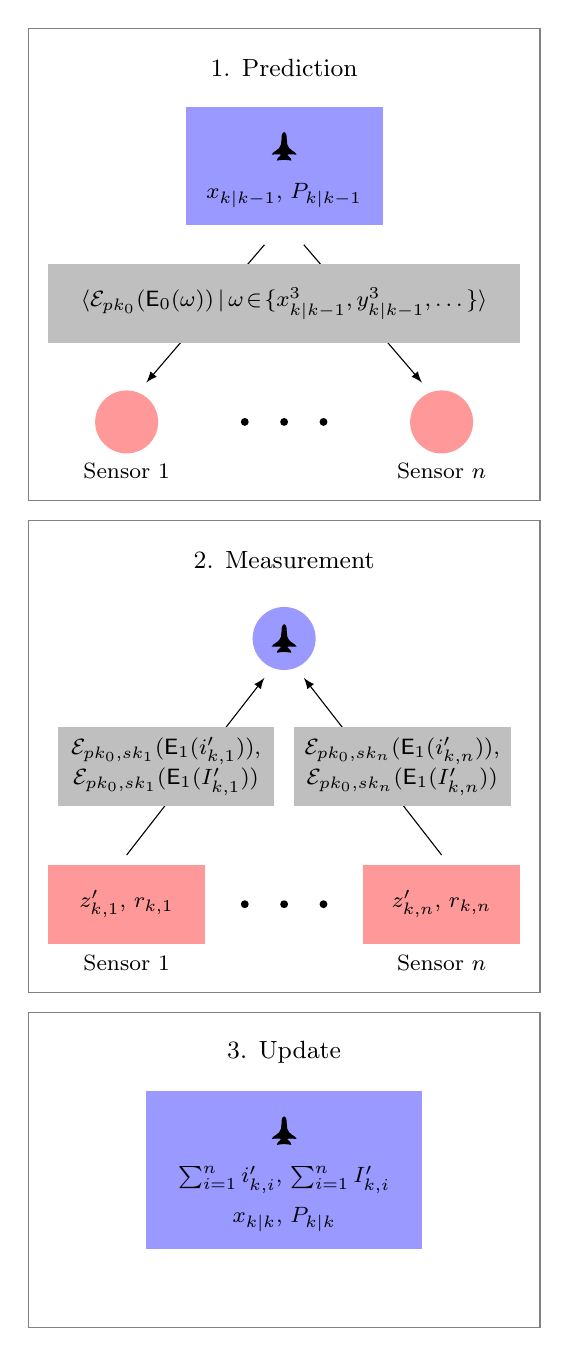
\begin{tikzpicture}[font=\footnotesize]
    % Prediction
    \draw [gray] (0,2) rectangle (6.5,8);
    \node at (3.25,7.5) {\small 1. Prediction};

    % Navigator
    \fill  [blue!40] (2,7) rectangle (4.5,5.5);
    \pic[xscale=0.22,yscale=0.3] at (3.25,6.6725) {plane};
    \node at (3.25,5.875) {$\rvec{x}_{k|k-1}$, $\mat{P}_{k|k-1}$};
    
    % Sensors
    \fill  (1.25,3) [red!40] ellipse (0.4 and 0.4);
    \node at (1.25,2.375) {Sensor $1$};
    \fill  (5.25,3) [red!40] ellipse (0.4 and 0.4);
    \node at (5.25,2.375) {Sensor $n$};
        
    \fill [black] (2.75,3) circle (0.05);
    \fill [black] (3.25,3) circle (0.05);
    \fill [black] (3.75,3) circle (0.05);
        
    % Arrows
    \draw [-latex] plot[smooth, tension=.7] coordinates {(3,5.25) (1.5,3.5)};
    \draw [-latex] plot[smooth, tension=.7] coordinates {(3.5,5.25) (5,3.5)};
    
    \fill [lightgray]  (0.25,5) rectangle (6.25,4);
    \node at (3.25,4.5) {$\langle\mathcal{E}_{pk_0}(\mathsf{E}_0(\rv{\omega})) \,|\, \rv{\omega} \!\in\! \{\rv{x}^3_{k|k-1}, \rv{y}^3_{k|k-1}, \dots\}\rangle$};
    
    
    % Measurement
    \draw [gray] (0,-4.25) rectangle (6.5,1.75);
    \node at (3.25,1.25) {\small 2. Measurement};
    
    % Navigator
    \fill  (3.25,0.25) [blue!40] ellipse (0.4 and 0.4);
    \pic[xscale=0.22,yscale=0.3] at (3.25,0.4225) {plane};
        
    % Sensors
    \fill  [red!40] (6.25,-3.625)  rectangle (4.25,-2.625);
    \node at (1.25,-3.875) {Sensor $1$};
    \fill  [red!40] (2.25,-3.625)  rectangle (0.25,-2.625);
    \node at (5.25,-3.875) {Sensor $n$};
    
    \node at (1.25,-3.125) {$\rv{z}'_{k,1}$, $\rv{r}_{k,1}$};
    \node at (5.25,-3.125) {$\rv{z}'_{k,n}$, $\rv{r}_{k,n}$};
    
    \fill [black] (2.75,-3.125) circle (0.05);
    \fill [black] (3.25,-3.125) circle (0.05);
    \fill [black] (3.75,-3.125) circle (0.05);
    
    % Arrows
    \draw [-latex] plot[smooth, tension=.7] coordinates {(1.25,-2.5) (3,-0.25)};
    \draw [-latex] plot[smooth, tension=.7] coordinates {(5.25,-2.5) (3.5,-0.25)};
    
    \fill [lightgray]  (0.375,-0.875) rectangle (3.125,-1.875);
    \node[align=center] at (1.75,-1.375) {$\mathcal{E}_{pk_0,sk_1}(\mathsf{E}_1(\rvec{i}'_{k,1}))$,\\$\mathcal{E}_{pk_0,sk_1}(\mathsf{E}_1(\mat{I}'_{k,1}))$};
    \fill [lightgray]  (3.375,-0.875) rectangle (6.125,-1.875);
    \node[align=center] at (4.75,-1.375) {$\mathcal{E}_{pk_0,sk_n}(\mathsf{E}_1(\rvec{i}'_{k,n}))$,\\$\mathcal{E}_{pk_0,sk_n}(\mathsf{E}_1(\mat{I}'_{k,n}))$};
    
    
    % Update
    \draw [gray] (0,-8.5) rectangle (6.5,-4.5);
    \node at (3.25,-5) {\small 3. Update};
    
    % Navigator
    \fill  [blue!40] (1.5,-5.5) rectangle (5,-7.5);
    \pic[xscale=0.22,yscale=0.3] at (3.25,-5.8275) {plane};
    \node at (3.25,-6.625) {$\sum_{i=1}^n \rvec{i}'_{k,i}$, $\sum_{i=1}^n\mat{I}'_{k,i}$};
    \node at (3.25,-7.125) {$\rvec{x}_{k|k}$, $\mat{P}_{k|k}$};
\end{tikzpicture}
\vspace{\baselineskip}
\caption{The summary of steps involved in our proposed privacy-preserving EIF.}
\label{fig:alg_steps}
\end{figure}

% 
% ##       ########    ###    ##    ##    ###     ######   ######## 
% ##       ##         ## ##   ##   ##    ## ##   ##    ##  ##       
% ##       ##        ##   ##  ##  ##    ##   ##  ##        ##       
% ##       ######   ##     ## #####    ##     ## ##   #### ######   
% ##       ##       ######### ##  ##   ######### ##    ##  ##       
% ##       ##       ##     ## ##   ##  ##     ## ##    ##  ##       
% ######## ######## ##     ## ##    ## ##     ##  ######   ######## 
% 

\subsection{Leakage} \label{subsec:leakage}
With the algorithm defined, we can analyse the localisation leakage when the strictly defined LCAO leakage is taken into account. We recall the assumptions on participant capabilities made in Section \ref{subsec:capabilities}. Consistent broadcasting is in line with the LCAO definition and required to guarantee the scheme's leakage. Honest-but-curious sensors are not required for scheme privacy, but avoid the possibility of malicious sensors gaining prior knowledge about remaining sensor measurements. This is possibly achieved by detecting changes in real measurements after reporting false measurements to the navigator. As stated in Section \ref{subsec:capabilities}, misbehaving sensors are a known problem which complicates homomorphic operations and active malicious sensors are not considered in the scope of this work.

The aggregation operation of our encryption scheme leaks the sums of sensor measurement vectors and matrices $\sum_{i=1}^n\rvec{i}'_{k,i}$ and $\sum_{i=1}^n\mat{I}'_{k,i}$. However, as stated in Remark \ref{rem:lcao_leakage}, weights chosen by a corrupted navigator mean that individual sums of coefficients can be leaked as well. That is, sums of coefficients in \eqref{eqn:hrz_linear_comb} and \eqref{eqn:hrh_linear_comb} (\textit{i.e.} $\sum_{i=1}^n2\rv{r}^{-1}_{k,i}$, $\sum_{i=1}^n-\rv{r}^{-1}_{k,i}s_{x,i}$, $\sum_{i=1}^n-2\rv{r}^{-1}_{k,i}s_{x,i}$, $\sum_{i=1}^n2\rv{r}^{-1}_{k,i}\rv{z}'_{k,i}$, \dots) are leaked to a corrupted navigator.

From the leaked coefficient sums, we see that all information private to the sensors and broadcast to the navigator, namely their modified measurements $\rv{z}'_{k,i}$, variance estimates $\rv{r}_{k,i}$ and locations $\vec{s}_i$, are present only in the sums
\begin{equation}
    \sum_{i=1}^n\rv{z}'_{k,i}\,,\ \sum_{i=1}^n\rv{r}_{k,i}\,,\ \sum_{i=1}^ns_{x,i}\ \textrm{and}\ \sum_{i=1}^ns_{y,i}\,.\label{eqn:localisation_leakage}
\end{equation}
From these sums and the definitions \eqref{eqn:modified_measurement} and \eqref{eqn:modified_measurement_variance_estimate}, we conclude that the navigator can \textit{at most} learn the sums of sensor private data, which in practice corresponds to the average sensor modified measurements, estimated variances and locations.
\begin{thm}
    In the context of our localisation scheme, leakage of the incorporated LCAO secure encryption scheme corresponds to the leakage of average sensor private information, given by the sums in \eqref{eqn:localisation_leakage}.
\end{thm}

% 
% 8888888b.  8888888888 .d8888b.  888     888 888    88888888888 .d8888b.  
% 888   Y88b 888       d88P  Y88b 888     888 888        888    d88P  Y88b 
% 888    888 888       Y88b.      888     888 888        888    Y88b.      
% 888   d88P 8888888    "Y888b.   888     888 888        888     "Y888b.   
% 8888888P"  888           "Y88b. 888     888 888        888        "Y88b. 
% 888 T88b   888             "888 888     888 888        888          "888 
% 888  T88b  888       Y88b  d88P Y88b. .d88P 888        888    Y88b  d88P 
% 888   T88b 8888888888 "Y8888P"   "Y88888P"  88888888   888     "Y8888P"  
%                                                                          
%                                                                          
%                                                                          
% 

\section{Simulation and Results} \label{sec:sim_and_results}
To demonstrate our proposed approach, we have implemented the algorithm in Section \ref{subsec:algorithm} and simulated the measurement and navigation of an object following a linear, time-invariant, process model in two-dimensional space. 

Code was written in the C programming language, using the MPI library \cite{OpenMPI2020} to support simultaneous computations by sensors and navigator as different processes. The OpenSSL library's \cite{OpenSSL2020} mask generation function MGF1 and hash function SHA256 were used to implement the required hash function $H$, while the Libpaillier library \cite{Libpaillier2010} was used for the implementation of the Paillier encryption scheme. Additionally, GNU libraries GSL \cite{GSLGNUScientific2019} and GMP \cite{GMPGNUMultiple2020} were used for algebraic operations and the handling of multiple-precision integers, respectively. Simulation execution was performed on a 3.00GHz Intel i7-9700 CPU, and run on the Windows Subsystem for Linux (WSL), where no real-time kernel was ensured but sufficiently consistent runtimes were observed for the purposes of our simulation.

Recalling the dependence of the modified measurement noise on the true measurement in \eqref{eqn:modified_measurement}, the noise distribution of the model changes with varying sizes of measurements. We considered four layouts with varying sensor distances when running our simulations to observe differences in estimation error when measurements are of different sizes. The considered layouts have been plotted and named in Figure \ref{fig:sim_layouts}.
\begin{figure}[htbp]
\begin{center}
    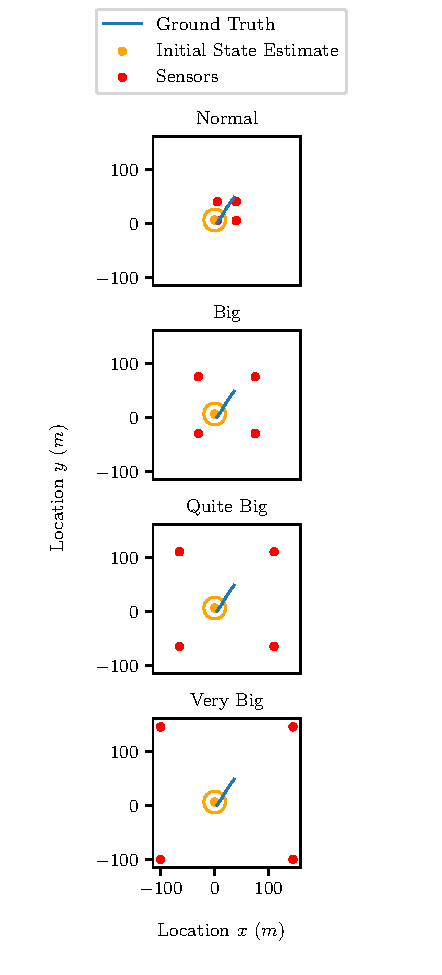
\includegraphics{images/layouts.pdf}
\end{center}
\caption{The considered layouts.}
\label{fig:sim_layouts}
\end{figure}
To evaluate the accuracy of our method, we have run $100$ simulations, all with $50$ filter iterations, for each of the sensors layouts with sensor measurement variances set to $r_i=5$ simulation distance units. Due to the large encoding modulus $N$, no notable advantage is gained when choosing a low fractional precision factor $f$, thus, $f=2^{32}$ was chosen to ensure minimal loss of precision when compared to the floating-point computations in the unencrypted EIF. The plotted average RMSE of our proposed method as well as that of the unencrypted EIF filter can be seen in Figure \ref{fig:sim_layout_errors}.
\begin{figure}[htbp]
\begin{center}
    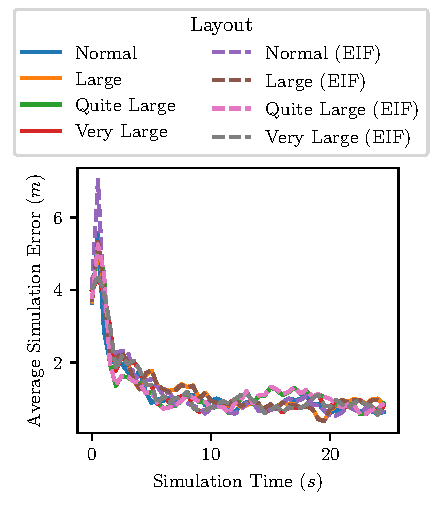
\includegraphics{images/layout_errors.pdf}
\end{center}
\caption{Filter error for different layouts.}
\label{fig:sim_layout_errors}
\end{figure}
From the results, it can be seen that sensor distance has little effect on the performance of the filter and that the measurement modification from Section \ref{subsec:range_measurement_mod} has a negligible effect when compared to a normal EIF filter. The robustness of the privacy-preserving method can be attributed to the conservativeness of variance estimates in \eqref{eqn:modified_measurement_variance_estimate} and the sufficiently large fractional precision parameter.

In addition to accuracy, computational requirements are an important factor in the adoption of novel cryptographic methods. Figure \ref{fig:sim_timing} shows the average simulation runtimes when encryption key bit lengths (\textit{i.e.} bit lengths of $N$) and the number of sensors are varied. Every plotted time is again the average of $100$ simulations, each running for $50$ filter iterations. 
\begin{figure}[htbp]
\begin{center}
    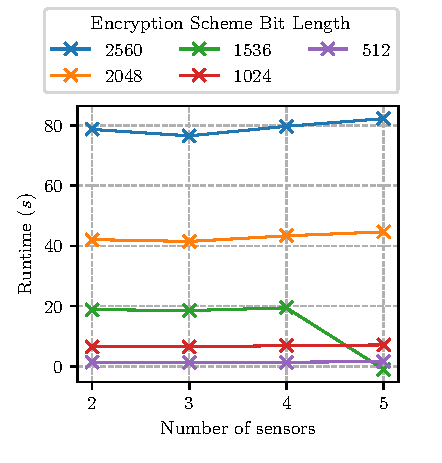
\includegraphics{images/timing.pdf}
\end{center}
\caption{Runtimes for varying key sizes and numbers of sensors.}
\label{fig:sim_timing}
\end{figure}
As sensor and navigator computations run in parallel, increases in runtime from additional sensors are primarily due to the longer aggregation operation at the navigator. The predominant computational cost is dependant on the encryption scheme key size, which must be chosen such that sufficient security is provided by the scheme. The current recommendation for a secure implementation relying on prime factorisation (difficulty of factorising $N$) is to use $2048$ bit-long keys \cite{barkerRecommendationPairwiseKey2019}.

% 
%  .d8888b.   .d88888b.  888b    888  .d8888b.  
% d88P  Y88b d88P" "Y88b 8888b   888 d88P  Y88b 
% 888    888 888     888 88888b  888 888    888 
% 888        888     888 888Y88b 888 888        
% 888        888     888 888 Y88b888 888        
% 888    888 888     888 888  Y88888 888    888 
% Y88b  d88P Y88b. .d88P 888   Y8888 Y88b  d88P 
%  "Y8888P"   "Y88888P"  888    Y888  "Y8888P"  
%                                               
%                                               
%                                               
% 

\section{Conclusion} \label{sec:conclusion}
To develop a model-based localisation algorithm which preserves navigator and sensor privacy, we first defined the novel notion of an LCAO secure encryption scheme and gave a provably secure implementation based on the Joye-Libert aggregation scheme. This scheme was then used in our proposed privacy-preserving EIF, where sensors compute measurement information homomorphically such that it can be privately used by a navigator. Our privacy-preserving estimation method may find uses in a variety of untrusted distributed localisation environments including airspaces and autonomous vehicle networks as well as those where alternative measurement models satisfying our defined linearity requirements can be applied. Possible future work in this topic includes the expanding of the LCAO security notion to \textit{ensure} that the same weights are broadcast to all sensors, the application of LCAO secure schemes to alternative measurement models and the exploring of implications behind an active sensor attacker model.

% Place acknowledgements
% here.
\begin{ack}                               
Partially supported by ZIM \dots
\end{ack}

% Include this if you use bibtex 
% and a bib file to produce the 
% bibliography (preferred). The
% correct style is generated by
% Elsevier at the time of printing.
\bibliographystyle{unsrt}
\bibliography{BibTeX/PrivateEIFLocalisation}

% Each appendix must have a short title.
% Sections and subsections are supported
% in the appendices.
\appendix
% 
%        d8888 8888888b.  8888888b.  8888888888 888b    888 8888888b. 8888888 Y88b   d88P 
%       d88888 888   Y88b 888   Y88b 888        8888b   888 888  "Y88b  888    Y88b d88P  
%      d88P888 888    888 888    888 888        88888b  888 888    888  888     Y88o88P   
%     d88P 888 888   d88P 888   d88P 8888888    888Y88b 888 888    888  888      Y888P    
%    d88P  888 8888888P"  8888888P"  888        888 Y88b888 888    888  888      d888b    
%   d88P   888 888        888        888        888  Y88888 888    888  888     d88888b   
%  d8888888888 888        888        888        888   Y8888 888  .d88P  888    d88P Y88b  
% d88P     888 888        888        8888888888 888    Y888 8888888P" 8888888 d88P   Y88b 
%                                                                                         
%                                                                                         
%                                                                                         
% 

\section{Indistinguishability under Chosen Plaintext Attack (IND-CPA)} \label{app:ind_cpa}
A public-key encryption scheme is defined by the tuple of algorithms $(\mathsf{Setup}, \mathsf{Enc}, \mathsf{Dec})$, defined as
\begin{description}
    \item[$\mathsf{Setup}(\kappa)$] On input of security paramater $\kappa$, generate public key $pk$ and secret key $sk$
    \item[$\mathsf{Enc}(pk, x)$] Encryption of value $x$ is computable using the public key $pk$, obtaining $\mathcal{E}_{pk}(x)$.
    \item[$\mathsf{Dec}(sk, \mathcal{E}_{pk}(x))$] Decryption of value $x$ is computable using the secret key $sk$.
\end{description}

The security game between attacker and challenger for IND-CPA security is given by
\begin{description}
    \item[Setup] The challenger runs the $\mathsf{Setup}$ algorithm and gives public key $pk$ to the attacker
    \item[Encryptions] The attacker may compute encryptions using the public key $pk$.
    \item[Challenge] Next, the attacker chooses two values
    \begin{equation*}
        x^{(0)} \text{ and } x^{(1)}
    \end{equation*}
    and gives them to the challenger. The challenger then chooses a random bit $b \in \{1,0\}$ and returns the encryption
    \begin{equation*}
        \mathcal{E}_{pk}(x^{(b)}).
    \end{equation*}
    \item[More Encryptions] The attacker can now compute more encryptions with the public key $pk$.
    \item[Guess] At the end, the attacker outputs a bit $b'$ and wins the game if and only if $b' = b$. The advantage of an attacker $\mathcal{A}$ is defined as
    \begin{equation*}
        \mathsf{Adv}^{IND-CPA}(\mathcal{A}) \coloneqq \left\lvert \Pr [b'=b] - \frac{1}{2}\right\rvert\,.
    \end{equation*} 
\end{description}

\section{Aggregator Obliviousness (AO)} \label{app:ao}
An aggregator oblivious encryption scheme is defined by the tuple of algorithms $(\mathsf{Setup}, \mathsf{Enc}, \mathsf{AggDec})$, defined as
\begin{description}
    \item[$\mathsf{Setup}(\kappa)$] On input of security paramater $\kappa$, generate public parameters $\mathsf{pub}$, the user private keys $sk_i,\,1\leq i \leq n$, and the aggregator's private key $sk_0=-\sum^n_{i=1}sk_i$.
    \item[$\mathsf{Enc}(t, sk_i, x^{(t)}_i)$] At instance $t$, user $i$ computes and obtains the encrypted value $y^{(t)}_i = \mathcal{E}_{sk_i}(x^{(t)}_i)$ using its secret key $sk_i$.
    \item[$\mathsf{AggDec}(t, sk_0, y^{(t)}_1,\dots,y^{(t)}_n)$] At instance $t$, the aggregator computes the aggregation of values $\sum^{n}_{i=1} x^{(t)}_i$ using its private key $sk_0$.
\end{description}

The security game between attacker and challenger for AO security is given by
\begin{description}
    \item[Setup] The challenger runs the $\mathsf{Setup}$ algorithm and gives public parameters $\mathsf{pub}$ to the attacker
    \item[Queries] The attacker can now submit queries that are answered by the challenger. The types of queries are:
    \begin{enumerate}
        \item \textit{Combine Queries:} The attacker chooses a tuple $(i,t,x^{(t)}_i$ such that for any two chosen combine query tuples $(i,t,x^{(t)}_i)$ and $(i',t',x^{\prime(t')}_{i'}$, the following condition holds:
        \begin{equation*}
            i = i' \wedge t = t' \implies x^{(t)}_{i} = x^{\prime(t')}_{i'}\,.
        \end{equation*}
        The attacker is then given back the encryption of the value $\mathcal{E}_{sk_i}(x^{(t)}_i)$ encrypted under the secret key $sk_i$.
        \item \textit{Compromise queries:} The attacker chooses $i$ and receives the secret key $sk_i$. The aggregator's secret key may also be compromised (when choosing $i=0$).
    \end{enumerate} 
    \item[Challenge] Next, the attacker chooses an instance $t^*$, and a subset of users $S \subseteq U$ where $U$ is the complete set of users for which no combine queries, for the instance $t^*$, and no compromise queries, are made for the duration of the game. The attacker then chooses two series of tuples
    \begin{equation*}
        \langle(i,t^*,x^{(t^*)(0)}_i)\,|\,i \in S\rangle
    \end{equation*}
    and
    \begin{equation*}
        \langle(i,t^*,x^{(t^*)(1)}_i)\,|\, i \in S\rangle\,,
    \end{equation*}
    and gives them to the challenger. In the case that $0 \in S$ (\textit{i.e.} the aggregator is compromised) and $S = U$, it is additionally required that
    \begin{equation*}
        \sum_{i\in S} x^{(t^*)(0)}_i = \sum_{i \in S} x^{(t^*)(1)}_i\,.
    \end{equation*}
    The challenger then chooses a random bit $b \in \{1,0\}$ and returns encryptions 
    \begin{equation*}
        \langle\mathcal{E}_{sk_i}(x^{(t^*)(b)}_i)\,|\,i\in S\rangle\,.
    \end{equation*}
    \item[More Queries] The attacker can now submit more queries, so long as the queries do not break the requirements in the Challenge stage. That is, $S \subseteq U$.
    \item[Guess] At the end, the attacker outputs a bit $b'$ and wins the game if and only if $b' = b$. The advantage of an attacker $\mathcal{A}$ is defined as
    \begin{equation*}
        \mathsf{Adv}^{AO}(\mathcal{A}) \coloneqq \left\lvert \Pr [b'=b] - \frac{1}{2}\right\rvert\,.
    \end{equation*} 
\end{description}

\end{document}